% This is a first shot at a somewhat comprehensive SATIrE manual. It is all
% in one file, which is not very nice. This file should be broken up into
% separate files for the chapters once the structure of the document has
% stabilized.

\documentclass[a4paper,12pt]{report}

\usepackage{graphicx}
\usepackage{listings}

\usepackage{longtable}
\usepackage{moreverb}
%\usepackage{fullpage}

\setlength{\parindent}{0pt}
\setlength{\fboxsep}{5pt}

\newcommand{\satire}[0]{SATIrE}

\input{manual_vars}

\newcommand{\msvector}[2]{{({#1},\ldots,{#2})}}
\newcommand{\outcomment}[1]{}
\newcommand{\hide}[1]{}
\def\makeactive#1{\catcode`#1 = \active\relax}
{\catcode`\^^I=\active %
 \catcode`\^^M=\active %
 \gdef\prologcode{ %
  \catcode`\^^I=\active %
  \catcode`\^^M=\active %
  \def^^I{\>} %
  \def^^M{\\[0pt]} %
 } %
}

\newenvironment{formula}
{%
\begin{displaymath}%
\begin{array}{rcl}%
}%
{%
\end{array}%
\end{displaymath}%
}%

\outcomment{
\newenvironment{example}
{%
\textbf{Example}.%
}%
{%
%
}%

\newenvironment{remark}
{%
\textbf{Remark}:%
}%
{%
%
}%

\newenvironment{proof}
{%
\textbf{Proof}:%
}%
{%
$\Box$%
}%
}

\newenvironment{PROG}                          % Prolog Umgebung
{
\begin{minipage}[t]{40ex}%
\prologcode\progfont%
\begin{quote}%
\begin{tabbing}%
\hspace{3ex}\=\hspace{3ex}\=\hspace{3ex}\=\hspace{3ex}%
\=\hspace{3ex}\=\hspace{3ex}\=\hspace{3ex}\=\hspace{3ex}\=\hspace{3ex}\=\hspace{3ex}\=\hspace{3ex}\=\hspace{3ex}\=\hspace{3ex}\kill}%
{\end{tabbing}%
\end{quote}%
\end{minipage}%
}

\newenvironment{PROGscriptsize}                          % Prolog Umgebung
{
\begin{minipage}[t]{40ex}%
\prologcode\scriptsize%
\begin{quote}%
\begin{tabbing}%
\hspace{3ex}\=\hspace{3ex}\=\hspace{3ex}\=\hspace{3ex}%
\=\hspace{3ex}\=\hspace{3ex}\=\hspace{3ex}\=\hspace{3ex}\=\hspace{3ex}\=\hspace{3ex}\=\hspace{3ex}\=\hspace{3ex}\=\hspace{3ex}\kill}%
{\end{tabbing}%
\end{quote}%
\end{minipage}%
}


%logic
\newcommand{\logand}[0]{\land}
\newcommand{\logor}[0]{\lor}
\newcommand{\lognot}[0]{\lnot}
\newcommand{\impl}[0]{\to}
\newcommand{\existsone}[0]{\exists!}
\newcommand{\notexists}[0]{\not\!\!\:\exists}

\newcommand{\ordner}[1]{ [Ordner {#1}]}

\newcommand{\pe}[1]{[{#1}]}
%sets
\newcommand{\setunion}[0]{\cup}
\newcommand{\setintersect}[0]{\cap}
\newcommand{\setdif}[0]{\backslash}
\newcommand{\tuple}[1]{({#1})}
\newcommand{\set}[1]{\{{#1}\}}
\newcommand{\pair}[2]{({#1},{#2})}
\newcommand{\tripel}[3]{({#1},{#2},{#3})}
\newcommand{\triple}[3]{({#1},{#2},{#3})}
\newcommand{\quadrupel}[4]{({#1},{#2},{#3},{#4})}

\newcommand{\cnodedef}[0]{\pair{ \set{ \pair{*}{\epsilon} } }{.} }
%\newcommand{\cnode}[0]{\diamond}
\newcommand{\cnodeset}[0]{\set{\diamond}}

%\newcommand{\bottomelement}{\tuple{\emptyset,\emptyset}}
\newcommand{\topelement}{\ensuremath{\top}}
\newcommand{\bottomelement}{\ensuremath{\perp}}
\newcommand{\dach} {\symbol{94}}
\newcommand{\deref}[1]{{#1}\dach}
\newcommand{\sname}[1]{[{#1}]}
\newcommand{\lname}[2]{[{#1},{#2}]}
\newcommand{\MSG}[0]{FSG }
\newcommand{\MSGpoint}[0]{FSG}
\newcommand{\MSGs}[0]{FSGs }
\newcommand{\MSGspoint}[0]{FSGs}
\newcommand{\MSGClass}[0]{\mathcal{\MSG}}
\newcommand{\Fcal}[0]{\mathcal{F}} % set of Functions, written as mathcal{F}.
\newcommand{\ffix}[0]{f.} % notation for fixpoint iteration
\newcommand{\mc}[1]{\multicolumn{3}{l|}{{#1}}} % multicolumn macro used in tabs for graphs
\newcommand{\kstring}[1]{\lceil {#1}]_k} % formal notation for k-truncated call strings (#1)
\newcommand{\nl}[1]{\ensuremath{\#{#1}}}

\newcommand{\edge}[1]{[{#1}]}

%\newcommand{\PP}[1]{{\em {#1}}}
\newcommand{\defeq}[0]{\stackrel{\mathrm{def}}{=}}

\newcommand{\exclude}[1]{}
\newcommand{\nsubset}{\not\subset}         %\\nsubset
%\newcommand{\textflorin}{\textit{f}}       %\\textflorin
\newcommand{\setB}{{\mathord{\mathbb B}}}  %\\setB
\newcommand{\setC}{{\mathord{\mathbb C}}}  %\\setC
\newcommand{\setN}{{\mathord{\mathbb N}}}  %\\setN
\newcommand{\setQ}{{\mathord{\mathbb Q}}}  %\\setQ
\newcommand{\setR}{{\mathord{\mathbb R}}}  %\\setR
\newcommand{\setZ}{{\mathord{\mathbb Z}}}  %\\setZ
\newcommand{\coloncolon}{\mathrel{::}}     %\\coloncolon
\newcommand{\lsem}{\mathopen{\lbrack\mkern-3mu\lbrack}}  %\\lsemantics
\newcommand{\rsem}{\mathclose{\rbrack\mkern-3mu\rbrack}} %\\rsemantics   
\newcommand{\pow}[1]{\mathcal{P}({#1})} % powerset of #1

\newcommand{\fullcirc}[0]{\bullet}
\newcommand{\heap}[0]{\mathcal{H}} % H (used for elements of the heap)
\newcommand{\nullref}[0]{\diamond} % box used as symbol for the reference value null
\newcommand{\nullnode}[0]{\ensuremath{\diamond}}
\newcommand{\recvar}[1]{\ensuremath{\bar{{#1}}}}
\newcommand{\ip}[1]{\ensuremath{\widehat{{#1}}}}% Notation for interprocedural entities 

\newcommand{\meetoperator}[0]{join operator }  % intraprocedural meet operator
\newcommand{\meet}[0]{\ensuremath{\sqcup}}  % intraprocedural meet operator
\newcommand{\imeet}[0]{\ip{\meet}}      % interprocedural meet operator
\newcommand{\bigmeet}[0]{\bigsqcup}        % big intraprocedural meet operator
\newcommand{\ibigmeet}[0]{\ip{\bigmeet}}% big interprocedural meet operator
\newcommand{\ifelse}[3]{                % if-else array for function definitions (3 parameters)
  \left\{\begin{array}{l@{\quad:\quad}l}%
      {#1} & {#2} \\%
      {#3} & \mbox{otherwise}%
    \end{array}%
  \right.}%

\newcommand{\longifelse}[4]{                % if-else array for function definitions (3 parameters)
  \left\{\begin{array}{l@{\quad:\quad}l}%
      {#1} & {#2} \\%
      {#3} & {#4} \\%
    \end{array}%
  \right.}%

\newcommand{\source}[1]{{\ttfamily #1}}
\newcommand{\progfont}[0]{\footnotesize}     % Zeichensatz 2 der Prologbeispiele
\newcommand{\mystring}[1]{"{#1}"}
\newcommand{\PP}[1]{{\progfont#1}\normalsize}
\newcommand{\ez}[0]{in }  % Das Elementzeichen
\newcommand{\anypath}[2]{{#1} *\to {#2}}
\newcommand{\nonnullpath}[2]{{#1} +\to {#2}}

\newcommand{\pathCd}[2]{{#1}{#2}}
\newcommand{\pathCa}[2]{{#1}{#2}}
\newcommand{\pathJ}[2]{{#1}{#2}}
\newcommand{\pathM}[2]{{#1}{#2}}
\newcommand{\code}[1]{{\textup\texttt {#1}}}

\newcommand{\ro}[0]{\ensuremath{\{\}}} % root in a graph

% new commands 2004

\newcommand{\emptystring}[0]{\epsilon}
\newcommand{\closurederivation}[0]{\rightarrow}
\newcommand{\derivationarrow}[0]{\Rightarrow}
\newcommand{\deriveone}[2]{{#1}\derivationarrow{#2}}
\newcommand{\derive}[2]{{#1}\stackrel{*}{\derivationarrow}{#2}}
\newcommand{\deriveminone}[2]{{#1}\stackrel{+}{\derivationarrow}{#2}}
\newtheorem{mydefinition}{Definition}
\newcommand{\classset}[0]{\mathcal{C}}
\newcommand{\gvar}[1]{\$$#1$}
\newcommand{\dollar}[0]{$\$$}
\newcommand{\markinfo}[1]{#1}

\title{SATIrE Manual}
\author{Markus Schordan, Gergo Barany, Adrian Prantl}

\pagestyle{headings}

\begin{document}
\maketitle

\chapter*{About this document}

This is the manual for SATIrE version \version.

\tableofcontents

\chapter{Introduction}
\label{chap:introduction}

SATIrE (\emph{Static Analysis Tool Integration Engine}) is a framework for
combining various tools for static analysis of computer programs. Its aim is
to support a wide range of source-level analyses and transformations
(including annotations and instrumentation) for C and C++ programs.

SATIrE is being developed at Vienna University of
Technology\footnote{\texttt{http://www.tuwien.ac.at}} and University of
Applied Sciences Technikum
Wien\footnote{\texttt{http://www.technikum-wien.at}}. It lives at:
\begin{center}
\verb|http://www.complang.tuwien.ac.at/satire/|
\end{center}

Major software products integrated in SATIrE are:
\begin{itemize}
\item the Program Analyzer Generator (PAG)
\item relevant parts of the ROSE source-to-source infrastructure and its
binding to the EDG C and C++ frontend
\item Termite
\end{itemize}

Additionally, SATIrE comes with a number of standard analyses that can be
used as building blocks when implementing custom program analyzers and
transformers.

Development of SATIrE has been funded within the ARTIST2 Network of
Excellence on Embedded Systems
Design\footnote{\texttt{http://www.artist-embedded.org}} and the ALL-TIMES
project\footnote{\texttt{http://www.all-times.org}}.

\chapter{SATIrE Tool Integration Architecture}

\section{Architecture - Conceptual View}
\label{sec:abstractarchitecture}

\begin{figure*}
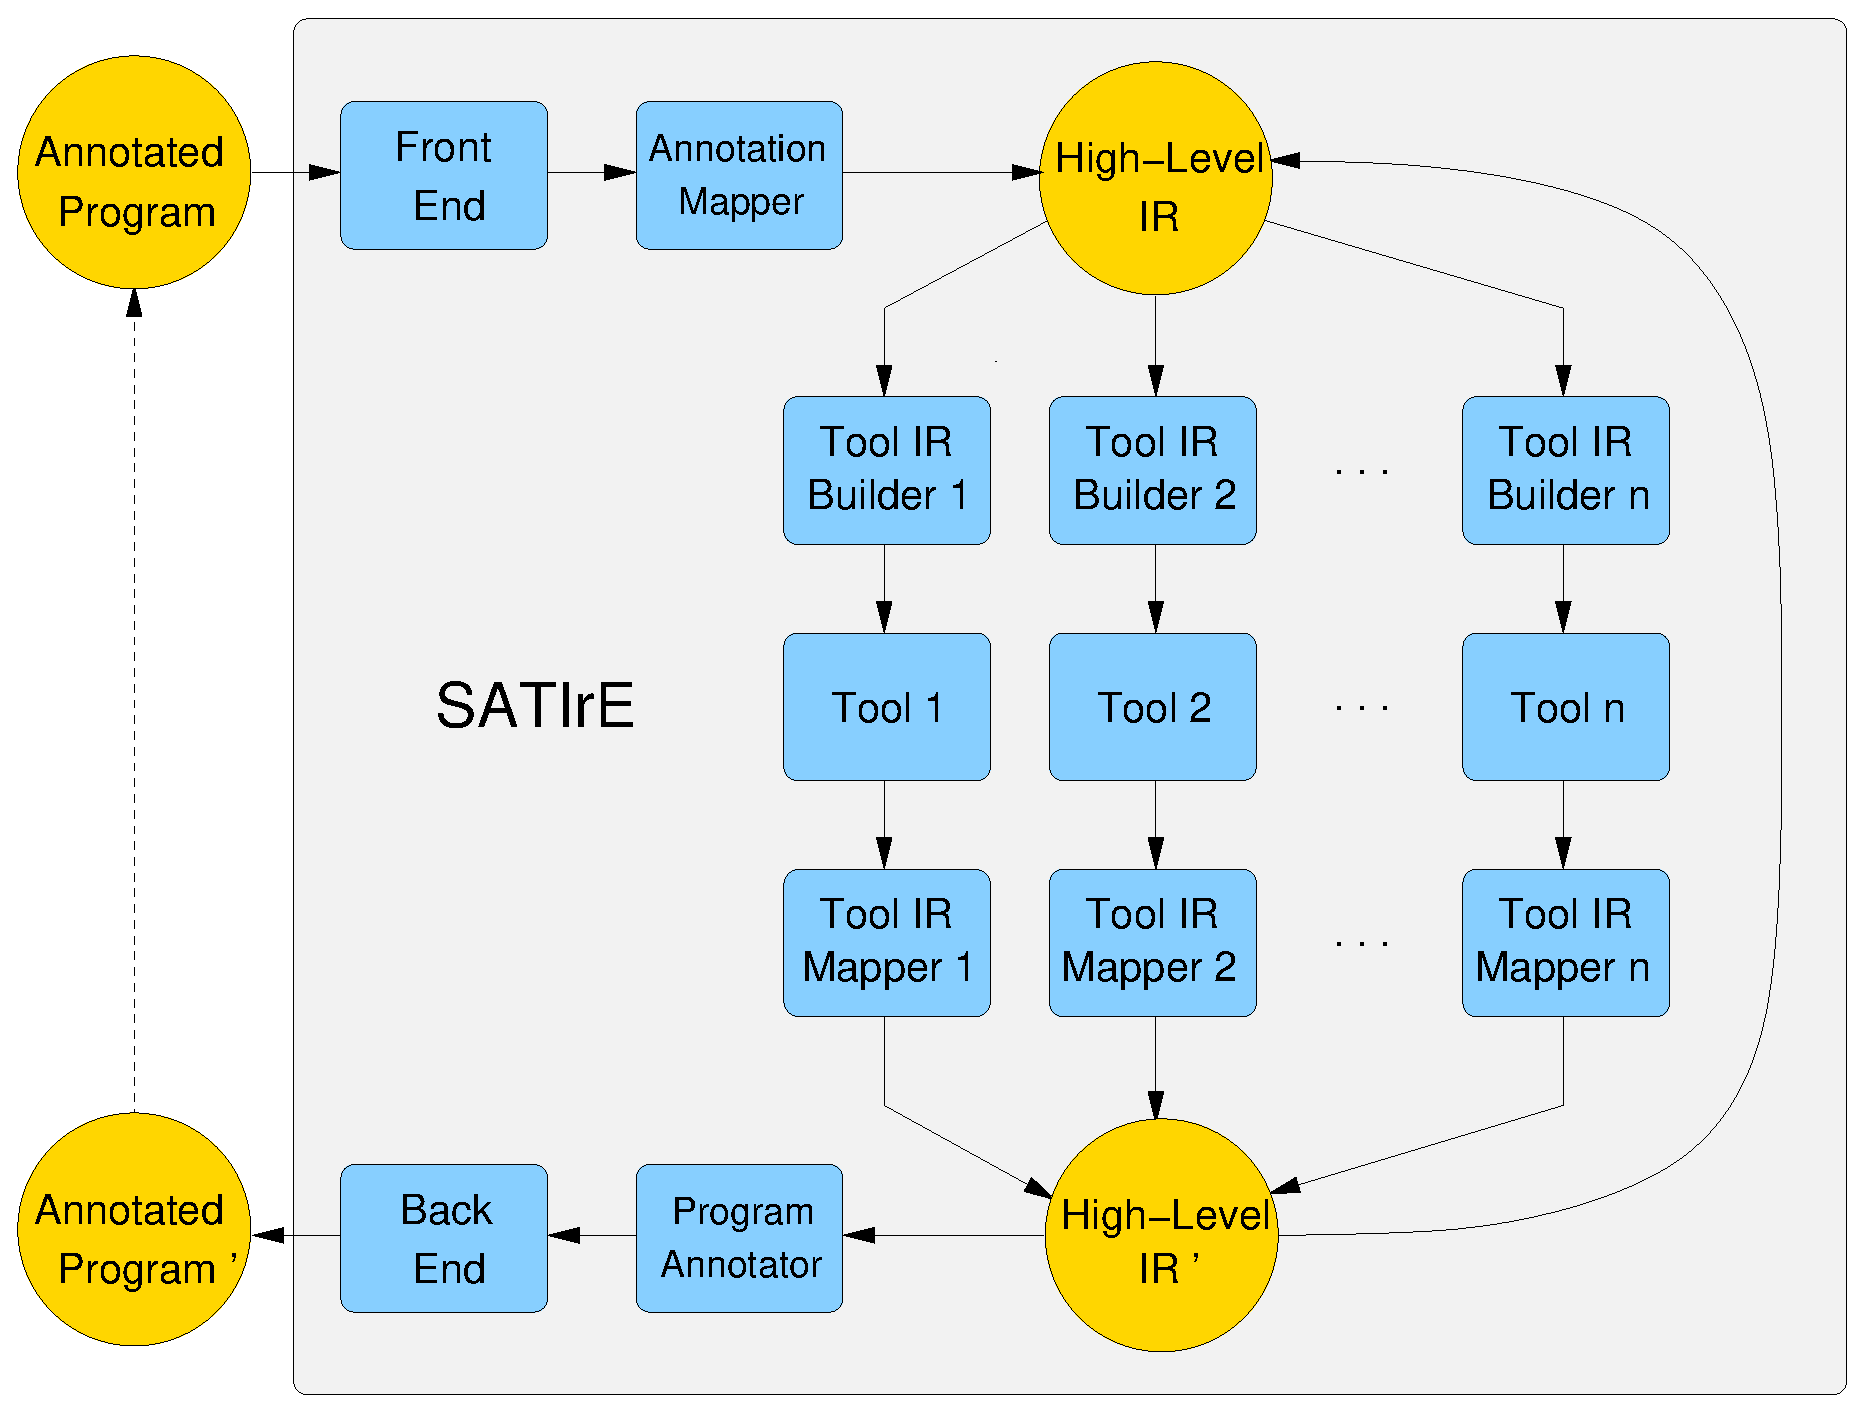
\includegraphics[scale=0.37]{abstractsatirearchitecture}
\caption{Static Analysis Tool Integration Engine Architecture}
\label{fig:abstractsatirearchitecture}
\end{figure*}

The architecture of the Static Analysis Tool Integration Engine
(\satire) for combining different analysis tools is shown at a conceptual level in Fig.~\ref{fig:abstractsatirearchitecture}. A central
aspect of the SATIrE approach is that information gathered about an input program
can be generated as annotation in the output program, and that the
output program can again serve as input program. This allows to make
analysis results persistent as generated source-code
annotations. Utilizing such annotations can also support whole
program optimization.

The architecture shown in Fig. \ref{fig:abstractsatirearchitecture} consists of the following kinds of components

\begin{description}
\item [Front End.] The (possibly annotated) program, $P$, is translated to a high-level intermediate representation (HL-IR).
\item [Annotation Mapper.] The annotations in $P$ are translated to annotations of the HL-IR.
\item [Tool IR Builder.] Each tool may require its own IR. The Tool-IR Builder creates the required Tool-IR by translating the HL-IR to the Tool-IR.
\item [Tool.] A tool analyzes or transforms its respective Tool-IR.
\item [Tool IR Mapper.] The Tool-IR mapper either maps the Tool's IR
back to High-Level IR or maps the computed information or results back
to locations in the HL-IR.
\item [Program Annotator.] The HL-IR annotations are translated to a representation in the source code. This can be comments, pragmas, or some specific language extension.
\item [Back End.] From the HL-IR an annotated program $P'$ (or an annotation file in ARAL format) is generated.
\end{description}

To allow a seamless integration of the tools, the Annotation Mapper,
Program Annotator, the Tool-IR Builders and Tool-IR Mappers are
offered by SATIrE. In Fig.~\ref{fig:abstractsatirearchitecture} the
solid back-edge represents an iterative application of the tools
within SATIrE.

\section{Architecture - Concrete View}
\label{sec:concretearchitecture}

To date we have integrated the Program Analyzer
Generator PAG~\cite{pag}, which generates analyzers from
high-level specifications, the LLNL-ROSE infrastructure for
source-to-source transformation of C++ programs~\cite{ROSE}, and
the term-based analyzer and transformation tool Termite, into \satire.
In the following sections we describe each integrated tool and give a
short overview of its integrated components.

\begin{figure*}
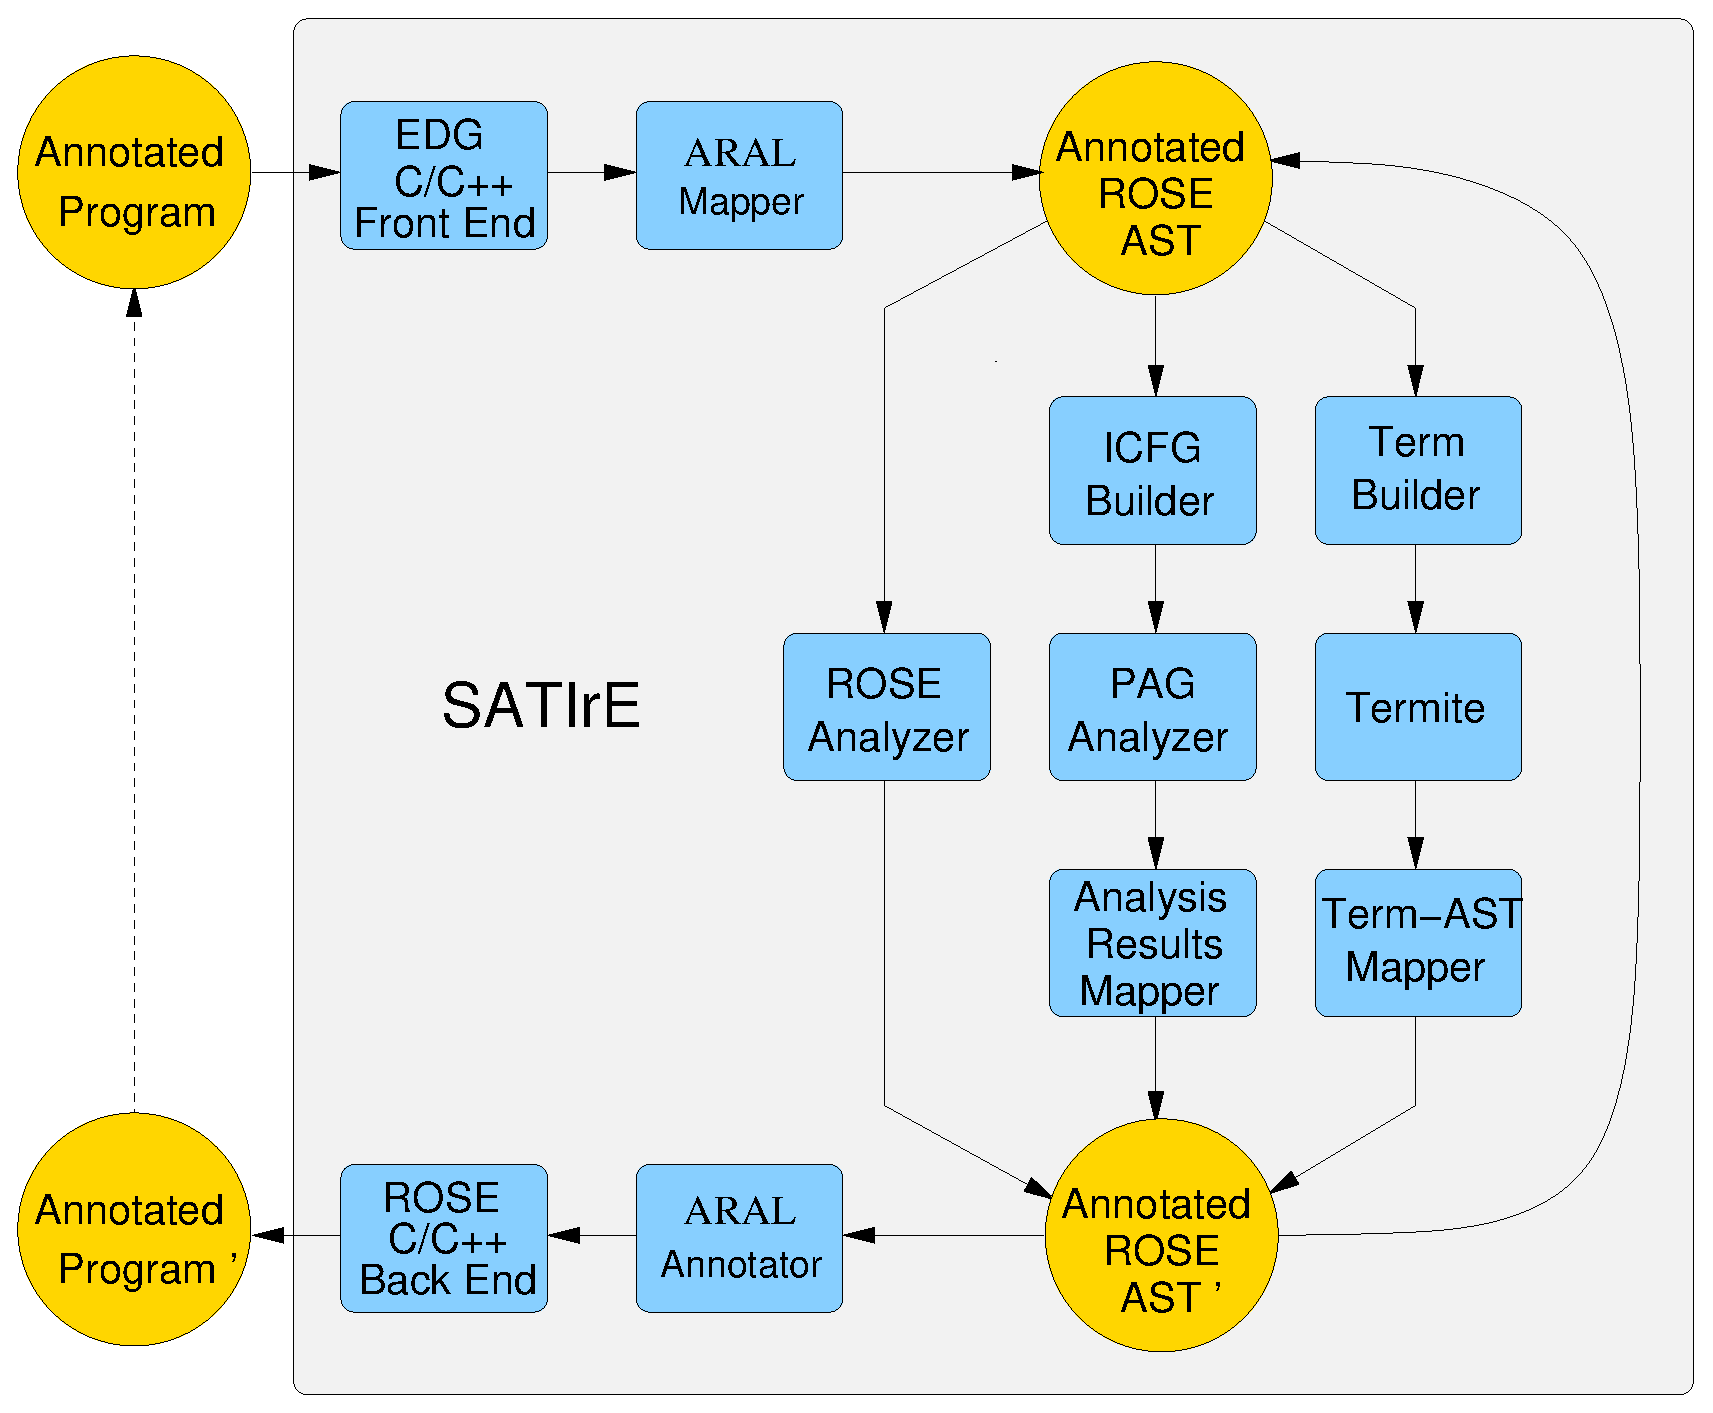
\includegraphics[scale=0.37]{concretesatirearchitecture}
\caption{SATIrE Architecture - Integrated Tools}
\label{fig:concretesatirearchitecture}
\end{figure*}

\subsection{LLNL-ROSE Integration}
\label{sec:ROSE}

The LLNL-ROSE infrastructure offers several components to build a
source-to-source translator. 
\outcomment{The ROSE Front End translates a C/C++
program to an object-oriented decorated abstract syntax tree. Several
different components can be used to build the midend of a translator:
to operate on the AST, a predefined traversal mechanism, a
restructuring mechanism, and an attribute evaluation mechanism can be
used to implement a transformation. A Back End is available for
unparsing the AST to a C++ program.
}
The ROSE components integrated into SATIrE are

\begin{description}
\item[C/C++ Front End.]
ROSE uses the Edison Design Group C++ Front End (EDG) \cite{EDG} to parse
C++ programs. The EDG Front End generates an abstract syntax tree (AST) and performs a full
type evaluation of the C++ program. The AST is represented as a C data
structure. ROSE translates this data structure into a decorated object-oriented
AST (ROSE-AST).

\item[Abstract Syntax Tree (ROSE-AST).]
The ROSE-AST represents the structure of the input program. It holds
additional information such as the type information for every
expression, exact line and column information, instantiated
templates, the class hierarchy (as it can be computed from the input
files), an interface that permits querying the AST, an an attribute
mechanism for attaching user-defined information to AST nodes.

\item[C/C++ Back End.]  The Back End unparses the AST and generates
C++ source code. It can be specified to unparse all included (header)
files or the source file(s) specified on the command line with
include-directives. This feature is important when transforming
user-defined data types.

\end{description}

\subsection{Program Analyzer Generator Integration}
\label{sec:analinterface}

The Program Analyzer Generator (PAG) from AbsInt, takes as input a
specification of a program analysis and generates an analyzer that
implements the analysis. The analyzer operates on an inter-procedural
control flow graph (ICFG) and provides the computed analysis results
as C data structure as well as a visualization of the ICFG and the
analysis results. The components necessary for a seamless integration
of PAG into SATIrE are

\begin{description}
\item [ICFG Builder.] Creates the inter-procedural control flow graph (ICFG) for a given ROSE-AST.
\item [PAG Analyzer.] Generated by the Program Analyzer Generator (PAG) from a user-defined analysis specification using the OPTLA language.
\item [Analysis Results Mapper.] Maps the analysis results back
to locations in the ROSE-AST and makes them accessible as ROSE-AST
annotations.
\end{description}

\outcomment{
PAG assumes a two-level intermediate representation for programs to
be analyzed: The analyzer generated by PAG requires the program to
be represented as a control-flow graph consisting of basic blocks
containing at least one statement each; for reasons of simplicity
our basic blocks consist of exactly one statement each, effectively
turning the graph from a basic-block graph into a single-instruction
graph
%~\cite{knoop98basicblock}.
Statements in basic blocks are taken
to be executed in order, blocks may have several predecessors and
successors according to the control flow. Edges between blocks may
be labeled to represent certain types of control flow, e.\,g.~true
and false branches. Blocks are organized in procedures, between
which only call and return edges are allowed.  A number of ICFG
access functions are implemented to enable the analyzer to
iterate over procedures, blocks, statements, and edges between
blocks. The statements themselves are
represented as abstract syntax trees.
}

Various types of ICFG attributes (for example numeric
labels for statements) and support functions are provided to the
analyzer by appropriate functions. Thus, the high-level
analysis specification can access any information the ROSE-AST
provides, such as types of expressions, the class hierarchy, etc.

\outcomment{
\subsection{Example}

A short example output of an automatically annotated program is shown
for the post-processed results of a shape analysis \cite{SRW98} in
Fig.~\ref{fig:example}. The shape analysis is specified using PAG, the
input program is a C++ program implementing a list reversal (and other
list operations). After translating the C++ program to the
corresponding ROSE-AST, SATIrE's ICFG builder creates the ICFG. Then the
PAG analyzer performs the shape analysis and the Analysis Results Mapper
maps the results back to the ROSE-AST. A post-processing of the
computed shapes generates may and must alias information. The
aliasing results are attached to the ROSE-AST nodes as must/may alias
annotations. The Program Annotator generates from the AST the annotations
as source code comments, and the ROSE Back End generates the annotated C++ code.

\outcomment{
\begin{sourcelisting}
SxET\\
VarSet             = set(str)\\
NodeSet            = set(VarSet)\\
HeapEdge           = VarSet * str * VarSet\\
HeapEdgeSet        = set(HeapEdge)\\
StackEdge          = str * VarSet\\
StackEdgeSet       = set(StackEdge)\\
Graph              = StackEdgeSet * HeapEdgeSet \\
ShapeGraph         = Graph * NodeSet\\
...\\
\\
DOMAIN \\
dfi              = flat(ShapeGraph)\\
\\
PROBLEM pointer\\
direction       : forward\\
carrier         : dfi\\
init            : bot\\
init_start      : lift((({},{}),{}))\\
equal           : eq\\
combine         : comb\\
retfunc         : comb\\
widening        : w\\
\end{sourcelisting}

\begin{sourcelisting}
// Support function for x = y; \\
assign_x_y::str,str,ShapeGraph -> ShapeGraph;\\
assign_x_y(x,y,((Ev0,Es0),is0)) =\\
  let Ev1=union({(za,msgc(x,y,Z))!!(za,Z) <-- Ev0},\\
              {(x,msgc(x,y,Z))!!(y1,Z) <-- Ev0, if y1=y});\\
      Es1={(msgc(x,y,Z1),sel0,msgc(x,y,Z2))!!(Z1,sel0,Z2) <-- Es0};\\
      is1={msgc(x,y,Z)!!Z <-- is0}; \\
  in\\
      ((Ev1,Es1),is1);\\
\end{sourcelisting}
}

\begin{figure}
\begin{verbatim}
class List* reverseList(class List* x)
{
  // pre must_aliases : {(l,x)} 
  // pre may_aliases : {(l,x)}  
  class List* y; 
  // pre,post must_aliases : {(l,x)}  
  // pre,post may_aliases : {(l,x)}  
  class List* t; 
  // post,pre must_aliases : {(l,x)}  
  // post,pre may_aliases : {(l,x)}  
  y = ((0)); 
  // post must_aliases : {(l,x)}  
  // post may_aliases : {(l,x)}  
  // pre must_aliases : {} 
  // pre may_aliases : {(l,t),(l,x),(l,y),(l,y->next),(t,y->next)}  
  while(x != ((0))) { 
    // pre must_aliases : {} 
    // pre may_aliases : {(l,t),(l,x),(l,y),(l,y->next),(t,y->next)}  
    t = y; 
    // post,pre must_aliases : {(t,y)}  
    // post,pre may_aliases : {(l,t),(l,x),(l,y),(l,y->next),(t,y)}  
    y = x; 
    // post,pre must_aliases : {(x,y)}  
    // post,pre may_aliases : {(l,t),(l,x),(l,y),(x,y)}  
    x = (x -> next); 
    // post,pre must_aliases : {(x,y -> next)}  
    // post,pre may_aliases : {(l,t),(l,y),(x,y->next)}  
    y -> next = t; 
    // post must_aliases : {} 
    // post may_aliases : {(l,t),(l,y),(l,y->next),(t,y->next)}  
  } 
  // post,pre must_aliases : {} 
  // post,pre may_aliases : {(l,t),(l,x),(l,y),(l,y->next),(t,y->next)}  
  t = ((0)); 
  // post,pre must_aliases :  {}
  // post,pre may_aliases : {(l,x),(l,y),(l,y->next)}  
  return y; 
  // post must_aliases : {} 
  // post may_aliases : {(l,x),(l,y),(l,y->next)}  
} 
\end{verbatim}
\caption{Example of a C++ program, annotated automatically with must/may
aliasing information which is computed by a post-processing phase from
the results of a shape analysis \cite{SRW98}. We extended the shape
analysis to an inter-procedural analysis. The analysis is specified by using PAG's specification language.}
\label{fig:example}
\end{figure}

The actual parameter in the call to the function \verb+reverseList+ is
\verb+l+, and is therefore aliased with the formal parameter
\verb+x+. When post analysis information (after a statement) and pre
analysis information (before a statement) is the same, it is shown in the same
line and preceded with \verb+post,pre+.
}

\subsection{Termite and Prolog Integration}

The integration of the tool Termite (i.e. Prolog) allows to specify a manipulation of the AST as term manipulation. The SATIrE components necessary for integration are

\begin{description}
\item[Term builder.] Creates a term representation for a given AST. The term representation is complete, meaning that it contains all information available in the AST. The term representation is stored in an external file.
\item[Termite - Prolog term manipulator] The term manipulation is specified as Prolog rules.
\item[Term-AST Mapper.] The transformed term is read in and translated
to a ROSE-AST.
\end{description}

More information on Termite can be found in the document termite.pdf.

%This approach has been successfully adopted within the COSTA project
%for performing Worst-Case Execution Time Analysis for a
%given C program. A detailed description can be found in \cite{adrian07}.

\chapter{SATIrE Analyzer Architecture}
\label{chap:analyzer}

This chapter describes the general structure of analyzers and their
interactions with the infrastructure provided by the SATIrE framework.

Note: Most of the identifiers described in this chapter live in the
\texttt{SATIrE} C++ namespace. They can be accessed by including the
\verb|<satire.h>| header.

\section{Command Line Flags}
\label{sec:command_line}

SATIrE contains a command line parser that reads options and input file
names and encapsulates them in an instance of the \texttt{AnalyzerOptions}
class.

The command line can be parsed using the
\begin{verbatim}
    AnalyzerOptions *extractOptions(int argc, char **argv);
\end{verbatim}
function. A list of all the flags understood by the command line parser, and
information on how to access this information from SATIrE analyzers, is
given in Appendix~\ref{appendix:command_line}.

\section{Program Input and Output}
\label{sec:program_io}

For each of the different program representations supported by SATIrE
(see Chapter~\ref{chap:program_representation}), there is a corresponding
function to build that representation from appropriate inputs. Each of these
functions takes an \texttt{AnalyzerOptions} object; besides specifying input
file names, this object contains additional options such as user requests
for sanity checks on the program representation, or for visualizations (of
the ICFG).

The ROSE AST (Section~\ref{sec:rose_ast}) can be built by calling:
\begin{verbatim}
    SgProject *createRoseAst(AnalyzerOptions *options);
\end{verbatim}
Note that this either reads source code, or a binary representation of a
previously constructed ROSE AST, depending on flags passed on the command
line.

The SATIrE ICFG (Section~\ref{sec:satire_icfg}) is built from a
ROSE AST by calling:
\begin{verbatim}
    CFG *createICFG(SgProject *astRoot, AnalyzerOptions *opts);
\end{verbatim}

Despite there being special functions for explicit creation of various
specialized program representations, it is often best to use SATIrE's
general high-level \texttt{Program} (Section~\ref{sec:satire_program})
class. Building a \texttt{Program} is performed by calling its
\begin{verbatim}
    Program(AnalyzerOptions *o);
\end{verbatim}
constructor.

Annotated or transformed programs can be output by calling the
\begin{verbatim}
    void outputProgramRepresentation(Program *program,
                                     AnalyzerOptions *options);
\end{verbatim}
function. This function will output the program as source code, as a binary
AST representation, or as a Termite term, depending on the command line
options. It will also output a visualization of the ICFG if requested.

Using these parts, one can build a very small SATIrE program that already
allows various forms of program analysis, visualization, and transformation:
\begin{verbatim}
    #include <satire.h>

    using namespace SATIrE;

    int main(int argc, char **argv)
    {
        AnalyzerOptions *options = extractOptions(argc, argv);
        Program *program = new Program(options);
        outputProgramRepresentation(program, options);
    }
\end{verbatim}

The tasks this program performs depend on the command line flags passed to
it by the user. Despite its power, this program is probably shorter than the
compiler command line you need to build and run it correctly :-) The
\verb|satire_driver| executable provided by SATIrE is just this program.

\section{Analyzer Interface}
\label{sec:analyzer_interface}

This section describes the general interface SATIrE analyzers are expected
to implement. This interface is the public interface of the abstract
\texttt{Analysis} class, from which all analyzers should be derived. There
is a more elaborate \texttt{DataFlowAnalysis} subclass for data-flow
analyzers generated using SATIrE and PAG; this class is described in more
detail in Chapter~\ref{chap:data_flow}.

The analyzer interface consists of several parts; first, there is a part for
meta information about the analyzer:
\begin{verbatim}
    virtual std::string identifier() const = 0;
    virtual std::string description() const = 0;
\end{verbatim}
The identifier is expected to be a single word naming the analyzer, while
the description is a brief human-readable summary of what the analyzer does.

The second part of the interface comprises methods for running the analysis
itself, and for performing actions depending on the results the analysis
computed:
\begin{verbatim}
    virtual void run(Program *program) = 0;
    virtual void processResults(Program *program) = 0;
\end{verbatim}
Note that these methods take as argument an instance of the general
\texttt{Program} class. This enables SATIrE to use a single analyzer
interface, while each analyzer can still decide which part of this program
representation (AST, ICFG, etc.) to run on. See
Chapter~\ref{chap:program_representation} for details on this issue.

Conceptually, the \texttt{run} method is meant to be a read-only analyzer
run that only collects information about the program and leaves the program
representation unchanged; the \texttt{processResults} method can then
annotate or transform the program as appropriate given those results. This
structure encourages modular analysis and transformation, but the separation
is not enforced by SATIrE.

The third part of the analyzer interface concerns dependencies between
analyzers. One of SATIrE's goals is modular construction of program
analyzers by combining, and building on, results from supporting analyses.
Where an analysis relies on results from other analyses, it must be ensured
that the supporting analyses are run before the client analysis. This is the
aim of the methods related to analyzer dependencies:
\begin{verbatim}
    void dependsOnAnalysis(Analysis *analysis);
    std::vector<Analysis *> &dependencies() const;
    void clearDependencies();
\end{verbatim}
The \texttt{dependsOnAnalysis} method is used to declare that the receiver
of the method call depends on results from the analyzer passed in the method
argument; the other two methods can be used to query the dependencies
declared so far, or to remove all of these dependencies.

\section{Running an Analyzer}
\label{sec:run_analyzer}

To run an analyzer with (or without) dependencies, rather than calling
its~\texttt{run} method directly, SATIrE's analysis scheduler should be
used. As far as users are concerned, this amounts to calling a single method
on the global scheduler object provided by SATIrE:
\begin{verbatim}
    analysisScheduler.runAnalysisWithDependencies(analysis,
                                                  program);
\end{verbatim}
This call is like calling
\begin{verbatim}
    analysis->run(program);
\end{verbatim}
except that the scheduler is aware of the dependencies between analyzers,
and ensures that they are satisfied.

If analyzer~\(A\) depends on analyzers~\(B\) and~\(C\), SATIrE's analysis
scheduler will thus ensure that~\(B\) and~\(C\) will be run---in some
unspecified order that is consistent with all the dependencies in the
system---before \(A\)'s \texttt{run} method is finally called by the
scheduler.

%\section{ARAL: Representing Analysis Results}
%\label{sec:aral}
%
%See the ARAL Manual for further information on ARAL (aralmanual.pdf)

\chapter{Program Representation in SATIrE}
\label{chap:program_representation}

This chapter describes the various ways SATIrE can represent programs under
analysis. The major representations are the ROSE abstract syntax tree~(AST),
SATIrE's interprocedural control flow graph~(ICFG), and the Termite term
representation of the AST. The \texttt{Program} class provides a unified
container for these representations.

\section{The ROSE AST}
\label{sec:rose_ast}

SATIrE uses the EDG C and C++ frontend provided with ROSE for parsing
programs. Thus, the AST used by ROSE is an important form of program
representation in SATIrE.\footnote{When support for clang is nearing
completion, SATIrE will offer the possibility to use clang instead of EDG as
the frontend. However, the representation built using this alternative
frontend will still use the ROSE AST classes.}

The ROSE AST is an object-oriented AST modeling the abstract syntax of a
given C or C++ program in great detail. ROSE programs can be traversed and
transformed in various ways; the reader is referred to the ROSE
documentation for details\footnote{\texttt{http://www.rosecompiler.org}}.
ROSE's program transformation capabilities and its unparser are used by
SATIrE to annotate ASTs and unparse them to annotated source code.

\section{The SATIrE ICFG}
\label{sec:satire_icfg}

SATIrE provides a representation of the program under analysis as an
inter-procedural control flow graph~(ICFG). The ICFG is designed to support
data-flow analysis using PAG, but it can also be used for other types of
analysis. The traversal mechanism provided by SATIrE (described below) makes
it possible to use the ICFG for flow-insensitive analysis in a way that is
similar to ROSE's AST traversals.

\subsection{Structure of the ICFG}
\label{sec:icfg_structure}

The ICFG is a directed graph consisting of nodes connected by labeled edges.
Each node contains a single statement, which can be a statement from the
original program, a transformed version of some original program statement,
or a new statement that does not directly correspond to a program statement,
but rather to a program point. Statements are represented using ROSE classes
as far as possible; statement types not occurring in ROSE are implemented by
subclassing ROSE's \texttt{SgStatement} class (via SATIrE's
\texttt{IcfgStmt} class).

Edges model (all) possible control flow, with labels providing information
on the type of flow: \verb|normal_edge| for regular flow; \verb|jump_edge|
for unconditional jumps; \verb|true_edge| and \verb|false_edge| for branches
(including loops); \verb|call_edge|, \verb|return_edge|, and
\verb|local_edge| for function calls, returns, and for connecting call and
return site in the caller, respectively. There are no interprocedural edges
except for calls and returns.

The following paragraphs list SATIrE's ICFG statements grouped by topic.

\paragraph{Variable scopes} The ICFG represents not only variable
declarations, but also `undeclarations' where variables go out of scope. The
corresponding statements are \verb|DeclareStmt| and \verb|UndeclareStmt|.
Compared to the ROSE AST, variable declarations are normalized such that
each \verb|DeclareStmt| declares exactly one variable; any initializers are
modeled using subsequent assignments.

\paragraph{Function boundaries} Functions (also called `procedures') in the
ICFG have explicit \verb|FunctionEntry| and \verb|FunctionExit| statements.
All calls and returns pass through these statements.

\paragraph{Function arguments} The ICFG makes argument passing explicit. It
introduces special global variables, collectively referred to as `tmpvars',
which behave similarly to argument registers in machine code. In particular,
before each function call node (see below), the ICFG contains a series of
nodes with \verb|ArgumentAssignment| statements. Each of these assigns the
value of some argument expression to a tmpvar. Within each function, the
entry node is followed by a sequence of \verb|ParamAssignment| statements
that assign each argument tmpvar to the corresponding parameter variable
inside the function.

\paragraph{Function return values} Returning values from functions is
similar to the handling of function arguments. Each \verb|return| statement
in the original program introduces an assignment to the global return
tmpvar. After the return from a function call, the ICFG introduces a
\verb|ReturnAssignment| statement that assigns the tmpvar's value to another
tmpvar specific to this call site. The original expression containing the
function call is rewritten in the ICFG to refer to the function's return
value through this tmpvar.

\paragraph{Function calls} Calls to functions that can be resolved
statically by the ICFG builder are represented by \verb|FunctionCall| and
\verb|FunctionReturn| ICFG statements. From the call node, there is a
\verb|call_edge| to the called function's entry node; that function's exit
node is connected to the caller's return node by a \verb|return_edge|. The
call and return nodes in the caller are also connected by a
\verb|local_edge|. Calls that the ICFG builder cannot resolve by itself are
modeled similarly, but using \verb|ExternalCall| and \verb|ExternalReturn|
statements; some analyzers may be able to discover call targets and add
appropriate edges to the ICFG (SATIrE's points-to analysis does this, see
Section~\ref{sec:analysis_pointsto}). Constructor and destructor calls are
modeled like normal function calls if they can be resolved; otherwise, they
are modeled using \verb|ConstructorCall| and \verb|DestructorCall|
statements, respectively.

\paragraph{Loops and branches} All \verb|for| loops are normalized to
\verb|while| loops with the same semantics. The point just after the loop
exit is marked with a \verb|WhileJoin| statement; the point where the paths
from an \verb|if| statement converge is marked with \verb|IfJoin|.

\paragraph{Short-circuiting operators} The control flow related to operators
that do not necessarily evaluate all of their arguments---the \verb|&&|,
\verb&||&, \verb|?:| operators---must be modeled explicitly in the ICFG.
This is done using the \verb|LogicalIf| statement. This statement is like a
regular \verb|if| statement; the node containing it has outgoing
\verb|true_edge| and \verb|false_edge| edges to nodes modeling evaluation of
subexpressions as appropriate. Intermediate results are stored in tmpvars.

\subsection{Accessing ICFG Information}
\label{sec:icfg_information}

The SATIrE ICFG is represented by an instance of SATIrE's \texttt{CFG}
class. The members of this class provide a lot of information about the
ICFG, but there is no nice public interface yet. The header file
\verb|cfg_support.h| provides access to the definition of this class and its
helpers.

As the ICFG was implemented to support data-flow analysis using PAG, SATIrE
provides a complete implementation of the ICFG query functions required by
PAG and documented in Chapter~9 of the PAG manual\footnote{PAG is not
available to the general public. You might be able to get a copy of PAG,
or at least its manual, by asking AbsInt nicely. PAG's homepage is at
\texttt{http://www.absint.de/pag/}.}. The \texttt{KFG} type
required by PAG is defined to be the \verb|CFG *| pointer type.

\subsection{Traversing the ICFG}
\label{sec:icfg_traversal}

SATIrE provides an ICFG traversal mechanism similar in spirit to ROSE's AST
traversals. This traversal is an efficient way to visit all statements in
the ICFG to perform flow-insensitive analysis. Note that statements are
visited in no particular order; in fact, even visits to statements in
different functions may be intermingled.

The traversal mechanism is implemented in the abstract
\texttt{IcfgTraversal} class in \verb|CFGTraversal.h|. Users must define a
derived class and provide a definition for at least this pure virtual
method:
\begin{verbatim}
    virtual void icfgVisit(SgNode *node) = 0;
\end{verbatim}
This method will be invoked by the traversal mechanism on each statement of
the ICFG. Additionally, it is also invoked for each initializer expression
provided for a global variable in the program. The ICFG traversal only
touches the roots of initializer expressions and ICFG statements; if you
wish to descend deeper into expressions and statements, you will need to use
some additional mechanism (e.\,g., ROSE's AST traversals).

In addition to the visit method, the following methods may also be
overridden:
\begin{verbatim}
    virtual void atIcfgTraversalStart();
    virtual void atIcfgTraversalEnd();
\end{verbatim}
These methods are called before the first time the visit method is called,
and after the last time the visit method has been called, respectively. The
default implementations do nothing.

As noted above, the order in which parts of the ICFG are visited may appear
chaotic. The traversal mechanism provides a number of member functions to
help in finding out what is being visited. The
\begin{verbatim}
    bool is_icfg_statement() const;
\end{verbatim}
function can be called from within the visit method to determine whether the
node being visited is a global initializer expression or a statement in the
ICFG. When visiting ICFG statements, the following methods may also be
called:
\begin{verbatim}
    int get_node_id() const;
    int get_node_procnum() const;
\end{verbatim}
These provide unique numeric identifiers for the current ICFG node, and for
the procedure the current node is part of.

The traversal itself is started by calling the following method of the
\texttt{IcfgTraversal} class on an ICFG:
\begin{verbatim}
    void traverse(CFG *icfg);
\end{verbatim}

%\section{Termite Terms}
%\label{sec:representation_termite}
%
%This section is not here yet. But a reference to Chapter~\ref{chap:termite}
%is here.

\section{SATIrE's \texttt{Program} class}
\label{sec:satire_program}

The \texttt{Program} class defined by SATIrE encapsulates the various forms
of program representation mentioned above. \texttt{Program} enables SATIrE
to use a single interface for all analyzers, even though internally they may
prefer different program representations. It has public members
corresponding to the options associated with the program, and the
representations that have been computed for it:
\begin{verbatim}
    AnalyzerOptions *options;
    SgProject *astRoot;
    CFG *icfg;
    PrologTerm *prologTerm;
\end{verbatim}

The \texttt{options} member is initialized by \texttt{Program}'s
constructor, which takes a mandatory \verb|AnalyzerOptions *| argument. This
constructor typically also ensures that the ROSE AST member is initialized.
However, the ICFG member will typically be \texttt{NULL} until it is needed;
analyzers that run on the ICFG should check this pointer and initialize it
using the \texttt{createICFG} function (Section~\ref{sec:program_io}) if
necessary.

The \texttt{prologTerm} member can point to a Termite term representing the
program. It is initialized by the \texttt{outputProgramRepresentation}
function if the option to output a Termite term is set.

\chapter{Writing Data-Flow Analyzers}
\label{chap:data_flow}

This chapter describes how to implement data-flow analyzers using PAG and
SATIrE. In this connection, PAG is used to generate a data-flow analyzer
from a functional specification, while SATIrE provides the program
representation (the ICFG) the analyzer runs on, as well as a number of
useful support functions, supporting types, and supporting analyses.

\section{Implementing an Analyzer}
\label{sec:pag_analyzer}

Implementation of a new data-flow analyzer starts with initializing an
analyzer directory using SATIrE's \texttt{newanalysis} script.
\texttt{newanalysis} can be called with an analyzer name provided on the
command line, in which case it will create a new directory with that name;
otherwise, it will use the current directory as the analyzer directory. In
any case, \texttt{newanalysis} creates a number of C++ code and header files
as well as some additional files.

\texttt{newanalysis} is also meant to create a Makefile for the analyzer.
However, this can only be done if it knows the name of the carrier type of
the analysis. This name can either be passed on the command line, or
\texttt{newanalysis} attempts to find it in the \texttt{.optla} file of the
analysis. If no \texttt{.optla} file has been written yet, the script will
not create a Makefile; you can invoke it again later, once the
\texttt{.optla} file is there.

How to implement the analysis specification itself is covered in detail in
the PAG manual. SATIrE supports both separate \texttt{.set} and
\texttt{.optla} files, as well as a single \texttt{.optla} file that also
contains all type information, as described in the PAG manual. Once (a
rudimentary version of) the analysis specification exists, and a Makefile
has been generated (possibly by a repeated invocation of
\texttt{newanalysis}), simply type \verb|make|. This will call PAG to
generate C code from the specification, compile that code and SATIrE's
support code, and build an executable with the same name as the analyzer
directory.

This executable is your analyzer program: It takes file names and additional
options on the command line and performs the analysis on the input programs.
The options determine how analysis results are visualized or made permanent.
See Appendix~\ref{appendix:command_line} on the command line flags you can
pass to the analyzer.

\section{SATIrE Support Features}
\label{sec:support_stuff}

This section lists all CFG attributes, types, and auxiliary functions
accessible from PAG analysis specifications when using the SATIrE system.
Declarations for all of these features are provided by SATIrE; the user need
not repeat these declarations.

\newcommand{\ttitemX}[1]{\item[\texttt{#1}]}
\newcommand{\ttitem}[1]{\ttitemX{#1} \mbox{} \\}

\subsection{Attributes}
\label{sec:support_attributes}

A CFG attribute is accessible from the analysis specification by name,
essentially like a variable that may have different values in different
places. See Chapter 12 of the PAG manual for details on the general concept.
The attributes are presented in a way that is similar to the syntax used in
the \texttt{.optla} file.


\paragraph{\texttt{GLOBAL} Attributes}
\begin{description}
\ttitem{globals: *VariableSymbolNT \#}
    A list of the global variables in the program. Types and initializers of
    global variables can be accessed via auxiliary functions, see below.

\ttitem{numtypes: unum \#}
    The number of different data types in the program. Types are associated
    with unique numbers that can be manipulated using auxiliary functions,
    see below.

\ttitem{numexprs: unum \#}
    The number of lexically different expressions in the program. Each
    expression is associated with a unique integer that can be manipulated
    using auxiliary functions, see below.
\end{description}

\paragraph{\texttt{ROUTINE} Attributes}
\begin{description}
\ttitem{procnum: snum \#}
    A unique numerical identifier for the current procedure. Procedure
    numbers are never negative.
\end{description}

\paragraph{\texttt{BLOCK} Attributes}
\begin{description}
\ttitem{label: snum \#}
    A unique numerical label for the block; as each block in SATIrE consists
    of exactly one statement, this can also be considered a unique label for
    each statement. Labels are never negative.
\end{description}

\paragraph{\texttt{POSITION} Attributes}
\begin{description}
\ttitem{position: snum \#}
    A numerical label for what PAG calls the `position' of the analysis
    information: The pair (procnum, position) is a unique (opaque)
    identifier for the interprocedural analysis context at the current point
    in the analysis.

\ttitem{context: ContextInfo \#}
    A ContextInfo object identifying the current interprocedural analysis
    context.
\end{description}

\subsection{Types}
\label{sec:support_types}

SATIrE defines a number of data types that can be used in PAG analysis
specifications. In contrast to the AST types defined in the syn file, the
types listed here behave more like built-in PAG types. In particular, they
can be used in the analyzer's carrier type.

The following types are provided as opaque identifiers for important data:

\begin{description}
\ttitem{VariableId}
    A unique identifier for each variable in the program. Two variables have
    the same identifier iff they are in fact the same variable. That is,
    variables with the same name, but in different scopes, have different
    \texttt{VariableId}s. There are conversion functions described below
    that convert \texttt{VariableSymbolNT}s or \texttt{VarRefExp}s to the
    variable's \texttt{VariableId}.

\ttitem{ExpressionId}
    A unique identifier for each expression in the program. Expressions are
    identified iff they are structurally equivalent, that is, they consist
    of identical operators applied to identical operands. Leaf variables are
    compared as \texttt{VariableId}s are, so two occurrences of \verb|a + b|
    in the program text will get the same \texttt{ExpressionId} iff they
    refer to the same variables \texttt{a} and \texttt{b}.

\ttitem{TypeId}
    A unique identifier for each type in the program. Types are identical if
    they are the same basic type or the same class type (i.\,e., have the
    same definition, structural equivalence does not suffice) or are derived
    from the same basic/class type using exactly the same specifiers and
    modifiers (pointer, \texttt{const}, etc.).

\ttitem{Location}
    An abstract `memory region' computed by points-to analysis for every
    program variable and other expression that refers to an object in
    memory, such as a pointer dereference, structure field access, etc. Two
    expressions may be aliases iff they correspond to the same
    \texttt{Location}; conversely, expressions that have different
    \texttt{Location}s are definitely not aliases.

    See Section~\ref{sec:analysis_pointsto} for more information on SATIrE's
    points-to analysis.

\ttitem{ContextInfo}
    An abstract object representing the current interprocedural analysis
    context. This is meant mainly to be passed to support functions that can
    provide context-sensitive information.
\end{description}

Comparisons for equality and total ordering relations for these types are
provided by SATIrE.

\subsection{Functions}
\label{sec:support_functions}

Auxiliary functions are functions provided by the SATIrE library to support
some common operations that would be impossible or very complicated to
implement in FULA. The definitions for these functions are automatically
linked against the generated analyzer. The declarations below are
automatically included in any analyzer created with SATIrE.

\begin{description}
\ttitem{is\_unary :: Expression -> bool;}
    test whether an Expression is a unary expression

\ttitem{is\_binary :: Expression -> bool;}
    test whether an Expression is a binary expression

\ttitem{is\_value :: Expression -> bool;}
    test whether an Expression is a value expression (a constant appearing
    in the source code)

\ttitem{unary\_get\_child :: Expression -> Expression;}
    get the operand expression of a unary expression

\ttitem{unary\_is\_prefix :: Expression -> bool;}
    determine whether the unary expression is a prefix expression

\ttitem{binary\_get\_left\_child :: Expression -> Expression;}
    get left child of a binary expression

\ttitem{binary\_get\_right\_child :: Expression -> Expression;}
    get right child of a binary expression

\ttitem{is\_subtype\_of :: Type, Type -> bool;}
    test whether type1 is a subtype of type2 (in the object oriented class
    hierarchy)

\ttitem{expr\_type :: Expression -> Type;}
    get the type of an expression

\ttitem{global\_get\_type :: VariableSymbolNT -> Type;}
    get the type of the global variable

\ttitem{global\_has\_initializer :: VariableSymbolNT -> bool;}
    test whether the global variable has an initializer expression

\ttitem{global\_get\_initializer :: VariableSymbolNT -> Expression;}
    get the initializer expression of the global variable

\ttitem{global\_has\_defining\_declaration :: VariableSymbolNT -> bool;}
    determine whether a global variable has a defining declaration in the
    program, or all declarations are extern

\ttitem{varsym\_varid :: VariableSymbolNT -> VariableId;}
    maps a variable symbol to its VariableId

\ttitem{varref\_varid :: Expression -> VariableId;}
    maps a VarRefExp to its VariableId; it is an error to call this with any
    other subtype of Expression!

\ttitem{expr\_exprid :: Expression -> ExpressionId;}
    maps the expression to its ExpressionId

\ttitem{exprid\_expr :: ExpressionId -> Expression;}
    maps the expression identifier to the actual expression it represents

\ttitem{is\_tmpvarid :: VariableId -> bool;}
    determines whether the variable identifier refers to a temporary
    variable introduced by SATIrE (for logical values, function return
    values, etc.)

\ttitem{is\_heapvarid :: VariableId -> bool;}
    determines whether the variable identifier refers to a heap variable
    introduced by SATIrE's points-to analysis (to name heap allocation
    sites)

\ttitem{varid\_str :: VariableId -> str;}
    gives the name of the variable with the given identifier

\ttitem{exprid\_str :: ExpressionId -> str;}
    gives the string representation of the expression with the given
    identifier

\ttitem{varid\_exprid :: VariableId -> ExpressionId;}
    maps a variable identifier to an expression identifier which denotes a
    VarRefExp for that variable

\ttitem{type\_typeid :: Type -> TypeId;}
    convert a type to its corresponding TypeId

\ttitem{typeid\_type :: TypeId -> Type;}
    convert a type identifier to the actual type it represents

\ttitem{typeid\_str :: TypeId -> str;}
    convert a type identifier to a string representation of the type

\ttitem{exprid\_typeid :: ExpressionId -> TypeId;}
    get the type identifier for a given expression identifier

\ttitem{add\_tmpvarid :: TypeId -> VariableId;}
    creates a new, unique temporary variable of the given type; this
    function returns different values for each call

\ttitem{is\_integer\_type :: Type -> bool;}
    determine whether the given type is some integer type

\ttitem{stmt\_asttext :: Statement -> str;}
    returns a string representing the structure of the given statement in a
    format very similar to PAG's pattern syntax

\ttitem{expr\_asttext :: Expression -> str;}
    returns a string representing the structure of the given expression in a
    format very similar to PAG's pattern syntax

\ttitemX{varid\_has\_location :: VariableId -> bool;}
\ttitem{varid\_location :: VariableId -> Location;}
    determine the abstract memory location corresponding to a variable;
    program variables have locations, SATIrE's temporary variables do not

\ttitem{varid\_has\_location\_cs :: VariableId, ContextInfo -> bool;}
    determine whether the variable has a location in a given context

\ttitemX{exprid\_has\_location :: ExpressionId -> bool;}
\ttitem{exprid\_location :: ExpressionId -> Location;}
    determine the abstract memory location corresponding to an expression,
    this can be a simple variable reference, but also a pointer dereference
    or other more complex expression; expressions that denote one of
    SATIrE's temporary variables, or expressions that do not denote an
    object in memory (an "lvalue") do not have locations

\ttitemX{varid\_location\_cs :: VariableId, ContextInfo -> Location;}
\ttitem{exprid\_location\_cs :: :: ExpressionId, ContextInfo -> Location;}
    context-sensitive variants of points-to support functions; the
    \texttt{ContextInfo} argument must be the current value of the
    \texttt{context} attribute (which is not directly available from support
    functions and must be passed as an argument if needed)

\ttitem{location\_varsyms :: Location -> *VariableSymbolNT;}
    returns the list of program variables stored in the given location

\ttitem{location\_funcsyms :: Location -> *FunctionSymbolNT;}
    returns the list of function symbols associated with the given function
    location

\ttitem{may\_be\_aliased :: Location -> bool;}
    determines whether the given location may be "aliased", i.e., whether
    some other location may hold a pointer to it

\ttitem{is\_array\_location :: Location -> bool;}
    determines whether the given location is an array

\ttitem{is\_ptr\_location :: Location -> bool;}
    determines whether the given location contains a pointer to some other
    location

\ttitem{dereference :: Location -> Location;}
    returns the pointed-to location of a given location that holds a pointer
\end{description}

\section{Abstract Syntax of SATIrE ICFG Statements}

The tree grammar describing the abstract syntax of the statements in the
ICFG is defined in the \texttt{syn} file in the SATIrE distribution. This is
the file PAG uses to generate its pattern matching code.

\section{Access to Call Strings}
\label{sec:call_strings}

SATIrE provides access to the call strings computed by PAG during
context-sensitive interprocedural analysis. After a PAG analysis has
completed, context information is added to the ICFG in its \texttt{contexts}
member. This is a container of \texttt{Context} objects as defined in
\verb|Context.h|. Each \texttt{Context} contains the corresponding procedure
and position identifiers as well as the call string itself: a sequence of
calls.

This feature is work in progress. In the future, it will be more powerful;
in particular, it will provide a way to access the caller's \texttt{Context}
from a given \texttt{Context}.

The \verb|--output-call-strings| command line flag instructs SATIrE
data-flow analyzers to print call string information. This call string
information looks something like this (the format is not set in stone):
\begin{verbatim}
    my_abs/0/0: main/613  ->  my_abs
    my_abs/0/1: main/613  ->  encode/233  ->  my_abs
    main/16/0: <spontaneous>
\end{verbatim}

Each line represents a context and the associated call string. The line
starts with the identifier of the context: the name of the current function,
its number, and the number of the context within this function. The call
string is a sequence of call sites leading to this function. Each call site
is identified by the name of the function containing the call, and the
identifier of the ICFG node containing the call statement. This ensures that
call sites can be uniquely identified even in functions that contain more
than one call to the same callee. Some contexts are identified as
`spontaneous'; this is typically the case for functions that are not called
from other functions in the program.

\chapter{Analyzers Provided by SATIrE}
\label{appendix:analyzers}

This appendix lists the analyzers that come with SATIrE to provide support
for other analyzers you wish to build.

\section{Data-Flow Analyzers}
\label{sec:analysis_dataflow}

SATIrE comes with a number of data-flow analyzers implemented using PAG.
Currently, these are:

\begin{center}
\begin{tabular}{l l p{.5\textwidth}}
Name & Carrier & Description \\
\hline
\texttt{constprop} & \verb|cp_LiftedState| &
    sketch of a constant folding/constant propagation analysis for
    integers\\
\texttt{interval} & \verb|itvl_State| &
    integer interval analysis\\
\texttt{sl2rd} & \verb|sl2rd_VarLabPairSetLifted | &
    reaching definitions analysis
\end{tabular}
\end{center}

\subsection{Using Provided Data-Flow Analyzers}
\label{sec:analysis_dataflow_use}

The predefined data-flow analyzers are included in the \texttt{libsatiredfa}
library, and the declarations of the corresponding C++ classes can be
included with the \texttt{satiredfa.h} header file. SATIrE's
\texttt{newanalysis} script will generate Makefiles and code skeletons that
use these automatically.

To run some predefined analyzer before your analysis, use SATIrE's analysis
scheduler (see Section~\ref{sec:run_analyzer}). At some point before the
\texttt{run} method of your analysis is called, you can declare a dependency
on the predefined analyzer using the \texttt{dependsOnAnalysis} method.

For instance, to use SATIrE's \texttt{constprop} analyzer before another
data-flow analyzer implemented using SATIrE, add the following statement
before the call to \texttt{run} in your analyzer's \texttt{main.C} file:

\begin{verbatim}
    analysis->dependsOnAnalysis(new DataFlowAnalysis(
                new SATIrE::constprop::Implementation()));
\end{verbatim}

The analysis scheduler will take care of running all analyzers in an order
that satisfies their dependencies.

You can access another analyzer's analysis data as described in the PAG
manual in the chapter entitled `Advanced Usage: Multiple Analyses'.
Essentially, each analysis has certain associated \texttt{NODE} and
\texttt{POSITION} attributes that another analysis can access from its
transfer functions.

Note that the exchange of analysis data is only guaranteed to work if all
involved analyzers use the same fixed-point iteration scheme. By default,
all analyzers generated with SATIrE use the same iterator
(\texttt{iterate1.t}).

\subsection{SATIrE Developers: Adding Analyzers}
\label{sec:analysis_dataflow_add}

To add a data-flow analyzer to the SATIrE library, follow these steps:

\begin{enumerate}
\item Add the analyzer specification in its own subdirectory under SATIrE's
\texttt{examples} directory. The analyzer \emph{must have an analysis
prefix} declared using \texttt{prefix:} in the problem description.
\item Add the type declarations for the analyzer's carrier type, and all of
the types it is constructed from, to the \texttt{pagoptions.set} file in
SATIrE's \texttt{src/analyzer/astaccess/satire} directory. To avoid name
clashes, you should add the analyzer's prefix to these type names.
\item Add the analyzer name to the definition of the \texttt{ANALYZERS}
variable in \texttt{src/analyzer/provided/dataflow/Makefile.am}. You can
ignore the rest o the Makefile; it will take care of building the analyzer,
including it in \texttt{libsatiredfa}, and installing the result.
\item Add a brief summary describing the analysis in the table above.
\item Do a \emph{very thorough} cleaning and rebuild of SATIrE, and test
whether other analyzers can access your analysis data.
\end{enumerate}

If all you are adding is a data-flow analyzer without any external support
functions (except those provided by SATIrE), this should work.

\section{Points-to Analysis}
\label{sec:analysis_pointsto}

%// The basic abstraction computed by this analysis is the Location, an
%// abstract memory region. Variables and functions (identified by their
%// respective symbols) live in Locations. Pointers are modeled by points-to
%// relations between Locations: each Location may have at most one "base
%// location", which is what it may point to. In this unification-based
%// analysis, Locations are merged when the same pointer may point to each of
%// them; that is, if the program contains the assignment sequence
%//      p = &a; p = &b;
%// then p's Location will point to a Location that contains both variables a
%// and b.
%// Each array is treated as a single object, i.e., all members live in the
%// same Location. It is assumed that array indexing and pointer arithmetic
%// always stay in the same object (as required by the Standard), so these
%// are safely ignored.
%// In contrast, structs are treated field-sensitively: Each struct instance
%// corresponds to a location, and each of its fields has its own location as
%// well. Such structs are collapsed when needed (if pointer arithmetic is
%// performed on a pointer to the structure or one of its members).
%
%// In principle, the heap can be modeled using the same abstractions.
%// However, this requires function summaries for allocation functions, which
%// are not here yet.
%
%    Points-to analysis must be activated using the
%    \texttt{--run-pointsto-analysis} command line flag; otherwise, analyzers
%    trying to access \texttt{Location}s will segfault. The analysis is a
%    variant of Steensgaard's flow-insensitive, context-insensitive analysis.
%    It works on C programs that are complete, i.\,e., do not call any
%    external functions. Casting and structures are supported. Pointer
%    arithmetic is supported as long as each pointer stays within one memory
%    region (array).


SATIrE comes with a flow-insensitive unification-based points-to analysis in
the spirit of Steensgaard~[cite\dots]. The analysis computes points-to
information for complete C programs, i.\,e., programs that do not call any
external functions. The analysis supports all C language features, including
typecasts, structures, arrays, pointer arithmetic, and function pointers. It
does not compute alias pairs; however, a client analysis could in principle
compute may-alias pairs from the points-to representation.

The basic analysis is context-insensitive; however, a context-sensitive
variant can be used with context-sensitive data-flow analyzers generated
using PAG.

\subsection{General Description of the Analysis}

The basic abstraction computed by the points-to analysis is the
\texttt{Location}, an abstract memory region. Variables and functions
(identified by their respective symbols) live in \texttt{Location}s.
Pointers are modeled by points-to relations between \texttt{Location}s: Each
\texttt{Location} may have at most one `base location', which is what it may
point to. In this unification-based analysis, \texttt{Location}s are merged
when the same pointer may point to each of them; that is, if the program
contains the assignments
\begin{verbatim}
    p = &a;
    p = &b;
\end{verbatim}
then \verb|p|'s \texttt{Location} will point to a \texttt{Location} that
contains both variables \verb|a| and \verb|b|.

Each array is treated as a single object, i.\,e., all members live in the
same \texttt{Location}. It is assumed that array indexing and pointer
arithmetic always stay in the same object (as required by the Standard), so
these are safely ignored. In contrast, structures are treated
field-sensitively: Each \texttt{struct} instance corresponds to a
\texttt{Location}, and each of its fields has its own \texttt{Location} as
well. Such structures are collapsed when needed (if pointer arithmetic is
performed on a pointer to the structure or one of its members).

Steensgaard's basic analysis is almost linear in the program size, taking
\(O(N \alpha(N))\), where \(N\) is some reasonable measure of the program
size and \(\alpha\) is an inverse of Ackermann's function. The SATIrE
implementation is a little more complex because of its more sophisticated
handling of structures. In practice, it is still very fast, however.

The points-to analysis runs on the ICFG, using the traversal mechanism
described in Section~\ref{sec:icfg_traversal}. It is most easily activated
by invoking the analyzer with the \texttt{--run-pointsto-analysis} command
line flag.

The \texttt{CFG} class contains a member that may be instantiated to a
points-to analyzer object:
\begin{verbatim}
    SATIrE::Analyses::PointsToAnalysis *pointsToAnalysis;
\end{verbatim}

The \texttt{PointsToAnalysis} class is defined in the \verb|pointsto.h|
header file. It implements the general analyzer interface described in
Section~\ref{sec:analyzer_interface}. The most important methods for
accessing points-to analysis results are:
\begin{verbatim}
    Location *expressionLocation(SgExpression *expr);
    Location *symbol_location(SgSymbol *sym);
\end{verbatim}
for access to \texttt{Location}s for expressions or variable/function
symbols, where two expressions/symbols may be aliases iff they are
associated with the same \texttt{Location} pointer;
\begin{verbatim}
    const std::list<SgSymbol *> &
    location_symbols(Location *loc) const;
\end{verbatim}
for access to all the symbols that are associated with a given
\texttt{Location};
\begin{verbatim}
    bool mayBeAliased(Location *loc) const;
\end{verbatim}
to find out whether there might be a pointer pointing to a given
\texttt{Location}; and
\begin{verbatim}
    Location *base_location(Location *loc);
    bool valid_location(Location *loc) const;
\end{verbatim}
to check what (if anything) a given \texttt{Location} may point to.

While the points-to analysis works fine, there is work in progress on making
it more precise and applicable to a wider range of programs. Precision can
be improved by adding context-sensitive elements; it will be possible to use
the analysis even for incomplete programs by providing summaries for
external functions. Using such summaries for allocation functions, the
latter will also allow analysis of points-to relationships on the heap.

\subsection{Context-Sensitive Extension}

SATIrE includes a context-sensitive variant of the points-to analysis
described above. In this variant, each function in the program is associated
with a number of interprocedural contexts, and is essentially analyzed
several times, once for each context. Argument and return locations of
function contexts are linked according to calling information between
contexts---distinct call sites of a function typically give rise to distinct
contexts, thus information from one call site of a function will usually not
be propagated to other call sites.

The context-sensitive points-to analysis is only availabe in conjunction
with data-flow analyzers generated using PAG, because SATIrE uses the
interprocedural contexts and call strings computed by PAG. This also means
that the degree of context sensitivity depends directly on the call string
length setting for PAG. The context-sensitive analysis is run automatically
if points-to analysis is enabled (using the \verb|--run-pointsto-analysis|
command line flag, for instance) and a context-sensitive data-flow analysis
attempts to use points-to information.

Due to this tight connection to PAG data-flow analyzers, the best way to
access context-sensitive points-to analysis data is by using the appropriate
support functions \verb|varid_location_cs| and \verb|exprid_location_cs|
(Section~\ref{sec:support_functions}) from within a data-flow analyzer.

\section{Loop Bounds Analysis}
\label{sec:analysis_loopbounds}

See termite.pdf for more Information on the provided loop bound analysis.

%\section{Coherence Analysis}
%\label{sec:analysis_coherence}

\chapter{ARAL: Analysis Results Annotation Language}

\section{Introduction}
\label{section:aral}
The analysis results annotation language (ARAL) is designed to be suitable
for annotating flow-sensitive and context-sensitive analysis
results. It allows to represent computed data of analysis tools, but
without putting restrictions on the semantics of an analysis. Clearly,
the annotations allow to represent analysis result data, but the semantics of
the data are defined for each analysis separately. For example, the
language is general enough to represent analysis information specified
in PAG's DATLA language \cite{pag}. Since PAG is integrated into
SATIrE this is a requirement for reusing any analysis information
computed with a PAG generated analyzer. ARAL consists of sets, lists,
tuples, maps, and some primitive data types. Additionally each
analysis information has an Analysis Identifier. This identifier
allows to associate semantics with the analysis information.

ARAL is designed to be a
general format that allows to exchange analysis information between
\satire and other tools. 

%Therefore it allows to exchange WCET
%analysis specific information, but also information for supporting
%analyses (e.g. interval analysis is an supporting analysis for loop
%bound analysis). This capability is necessary for use case R.

ARAL is suitable for annotating flow-insensitive as well as
flow-sensitive and context-insensitive as well as context-sensitive
analysis results. It allows to represent computed data of analysis
tools, but without putting restrictions on the semantics of an
analysis. Clearly, the annotations allow to represent analysis result
data, but the semantics of the data are defined for each analysis
separately. For example, the language is general enough to represent
analysis information specified in AbsInt's PAG DATLA language. Since
PAG is integrated into \satire{} this is a requirement for reusing any
analysis information computed with a PAG generated analyzer. ARAL
consists of sets, lists, tuples, maps, and some primitive data
types. Additionally each analysis information has an Analysis
Identifier. This identifier allows to associate semantics with the
analysis information.

%To associate the analysis information with a program fragment
%a label and a mapping exists to associate the analysis information with
%a program fragment.

%\outcomment{

\section{Language}

%TODO: the language shall be described by discussion of type-system
%and data-representation only. The mapping and file structure shall be
%explained in the file format chapter. ARAL is for administration
%of analysis results (combination of files etc.). A COMPUTATION section will allow compact representation of analysis results.\\

ARAL is a strictly typed language. A data element can only have
exactly one type and there is no void type. For a proper use of the
language it is important to be aware of the concept of the mapping
section and the result section(s). In a result section analysis data
is represented independent from the intermediate representation on
which is was computed. The mapping section defines how the analysis
information of a result section is associated with locations in a
source code of a program and similarly, how it is associated with
locations in an intermediate representation. The two different kinds
of sectionos support a separation of concerns: the analysis data
itself and how it is associated with locations in a program. The
locations are labeled, and those labels are used in the data
section. For expressions (and its subexpressions) IDs are computed
that those IDs are used in the DATA section. A mapping section can
provide information on how to map the IDs to source code constructs.

\subsection{ARAL Grammar}

{
\newcommand{\regexstar}[1]{\{~#1~\}$^*$}
\newcommand{\regexplus}[1]{\{~#1~\}$^+$}
\newcommand{\regexgroup}[1]{\{~#1~\}}
\newcommand{\regexopt}[1]{[~#1~]}
\newcommand{\lexrange}[2]{\underline{#1}-\underline{#2}}
\newcommand{\lb}[0]{\underline{(}~}
\newcommand{\rb}[0]{\underline{)}}
\newcommand{\comma}[0]{\underline{,}~}
\newcommand{\garrow}[0]{$\rightarrow$}

\newenvironment{GRAMMAR}                          % Prolog Umgebung
{
\begin{minipage}[t]{40ex}%
\prologcode\progfont%
\begin{quote}%
\begin{tabbing}%
\hspace{3ex}\=\hspace{3ex}\=\hspace{3ex}\=\hspace{3ex}%
\=\hspace{3ex}\=\hspace{4ex}\=\hspace{3ex}\=\hspace{3ex}\=\hspace{3ex}\=\hspace{3ex}\=\hspace{3ex}\=\hspace{3ex}\=\hspace{3ex}\kill}%
{\end{tabbing}%
\end{quote}%
\end{minipage}%
}

This subsection gives a precise definition of the ARAL syntax. The
grammar is specified in the usual notation for context-free grammars,
plus some convenient abbreviations:

\begin{itemize}
\item Non terminals start with a capital letter.
\item Terminals are underlined.
\item Optional constructs are enclosed in square brackets: [ Optional ]
\item Alternatives are separated by $\mid$: A $\mid$ B
\item Zero or more occurrences are enclosed in curly braces with a star: \regexstar{zero or more}
\item One or more occurrences take a '+': \regexplus{ one or more}
\item Sequences of constructs are separated by spaces.
\item Ranges are written with a dash, e.g. \underline{0}-\underline{9}.
\item Braces indicate grouping, e.g. \{ A $\mid$ B \} C
\item Some productions are explained with comments: \% comment.
\end{itemize}

Primitive tokens are 'Number' (\regexplus{\underline{0}-\underline{9}}) and identifiers, 'Id' (\regexgroup{\lexrange{A}{Z}$\mid$\lexrange{a}{z}}\regexstar{\underline{\_}$\mid$\lexrange{A}{Z}$\mid$\lexrange{a}{z}$\mid$\lexrange{0}{9}}).
ARAL comments start with a double slash and end at the end of the current line. Whitespace may be inserted anywhere between tokens.

The grammar productions can be found in Fig.~\ref{fig:annotationfileformat},\ref{fig:aralone}, \ref{fig:araltwo}.

\begin{figure}[!ht]
\begin{GRAMMAR}
{AralFile}      \>\>\>\>\>\garrow\> \underline{ANALYSIS} 
                 \>\>\>\>\> \> \regexopt{ConfigSection}
                 \>\>\>\>\> \> \regexopt{MappingSection} 
                 \>\>\>\>\> \> \regexopt{ResultSection} 
                 \>\>\>\>\> \>       \underline{END}

{ResultSection}    \>\>\>\>\>\garrow\> \underline{RESULT}
                 \>\>\>\>\> \> NameSection
                 \>\>\>\>\> \> TypeSection 
                 \>\>\>\>\> \> DataSection 
                 \>\>\>\>\> \> \underline{END}

{NameSection}    \>\>\>\>\>\garrow\> \underline{NAME} AnalaysisIdent

{ConfigSection}  \>\>\>\>\>\garrow\> \underline{CONFIG} ConfigType \underline{:} ConfigData \underline{;}

{MappingSection}  \>\>\>\>\>\>\garrow\> \underline{MAPPING} \regexstar{\underline{map}\lb~FromType\comma~Type \rb ~\underline{:} Map \underline{;}} 
                  \>\>\>\>\>\>\% keyword IDMAP is deprecated

{FromType}       \>\>\>\>\>\garrow\> Label
                 \>\>\>\>\> \> $\mid$ ProgId

{TypeSection}    \>\>\>\>\>\garrow\> \underline{TYPE} \regexstar{TypeDef} \regexopt{\underline{$\langle$} ContextType \underline{$\rangle$}} AnnotType 

{DataSection}    \>\>\>\>\>\garrow\> \underline{DATA} \regexstar{AnnotData}

{AnalysisIdent}  \>\>\>\>\>\garrow\> Id
{ConfigType}     \>\>\>\>\>\garrow\> Type
{ConfigData}     \>\>\>\>\>\garrow\> Data
{AnnotType}      \>\>\>\>\>\garrow\> Type
{ContextType}    \>\>\>\>\>\garrow\> Type

{TypeDef}        \>\>\>\>\>\garrow\> Id \underline{=} Type \underline{;}

{Type}           \>\>\>\>\>\garrow\> \underline{set}\lb Type \rb
                 \>\>\>\>\> \> $\mid$ \underline{list}\lb Type \rb
                 \>\>\>\>\> \> $\mid$ \underline{tuple}\lb Type$_1$,...,Type$_n$ \rb
                 \>\>\>\>\> \> $\mid$ \underline{flat} \lb Type \rb
                 \>\>\>\>\> \> $\mid$ \underline{lift} \lb Type \rb
                 \>\>\>\>\> \> $\mid$ \underline{map} \lb Type \comma Type \rb
%                 \>\>\>\>\> \> $\mid$ \underline{enum} \lb Id \regexstar{\comma Id} \underline{$\mid$} \regexopt{Edge \regexstar{\comma Edge}} \underline{$\mid$} Id \underline{$\mid$} Id \rb
                 \>\>\>\>\> \> $\mid$ \underline{label}
                 \>\>\>\>\> \> $\mid$ \underline{constraint}
                \>\>\>\>\> \> $\mid$ \underline{string}
                \>\>\>\>\> \> $\mid$ \underline{int(} Number \underline{)}
                 \>\>\>\>\> \> $\mid$ IdNumber
                 \>\>\>\>\> \> $\mid$ Basic
                 \>\>\>\>\> \> $\mid$ ProgId

{Label}           \>\>\>\>\>\garrow\> $\texttt{\underline{@}}$Number

{IdNumber}       \>\>\>\>\>\garrow\> $\underline{\texttt{\#}}$Number

%Edge             \>\>\>\>\>\garrow\> Id $\leq$ Id
\end{GRAMMAR}
\caption{Grammar for the ARAL Annotation File Format (Part 1, see Fig. \ref{fig:aralone} for productions of AnnotData, Basic, ProgId, and Map)}
\label{fig:annotationfileformat}
\end{figure}

\begin{figure}[!ht]
\begin{GRAMMAR}
{AnnotData}      \>\>\>\>\>\garrow\> LocationSpec FlowSpec InfoElement \underline{;}

{LocationSpec}   \>\>\>\>\>\garrow\> [ ExpPath ] LocSpecTarget

{LocSpecTarget}  \>\>\>\>\>\garrow\>Label
                 \>\>\>\>\> \>$\mid$ \underline{(} Label \underline{,} Label \underline{)} \hspace{2cm}\% not implemented 
                 \>\>\>\>\> \>$\mid$ \underline{program}
                 \>\>\>\>\> \>$\mid$ \underline{file} \underline{(}  String \underline{)} 
                 \>\>\>\>\> \>$\mid$ \underline{function} \underline{(}  String \underline{)} 

{ExpPath}        \>\>\>\>\>\garrow\> \underline{call} \underline{(} Number \underline{)} \underline{:} \regexopt{\underline{param} \underline{(} Number \underline{)}\underline{:}} \% not implemented

{FlowSpec}       \>\>\>\>\>\garrow\> \underline{pre} $\mid$ \underline{post} $\mid$ \underline{noflow}

{InfoElement}    \>\>\>\>\>\garrow\> \regexopt{\underline{$<$}Context\underline{$>$}} Data \regexstar{\underline{,} \underline{$<$}Context\underline{$>$} Data}

{Basic}          \>\>\>\>\>\garrow\> \underline{bool} $\mid$ \underline{string} $\mid$ \underline{real} $\mid$ NumRange

{ProgId}         \>\>\>\>\>\garrow\> \underline{funcid} $\mid$ \underline{declid} $\mid$ \underline{stmtid} $\mid$ \underline{exprid} $\mid$ \underline{varid}


{Context}        \>\>\>\>\>\garrow\> Data

{NumRange}       \>\>\>\>\>\garrow\> \underline{[} NumExp \underline{..} NumExp \underline {]} \% not implemented

{NumExp}         \>\>\>\>\>\garrow\> [-] Number
                 \>\>\>\>\> \>$\mid$ NumExp NumOperator NumExp
                 \>\>\>\>\> \>$\mid$ [-] \lb~NumExp \rb

{NumOperator}    \>\>\>\>\>\garrow\> \underline{+} $\mid$ \underline{-} $\mid$ \underline{*} $\mid$ \underline{/} $\mid$ \underline{\%} $\mid$ \underline{\symbol{"5E}}

\end{GRAMMAR}
\caption{ARAL Grammar (Part 2)}
\label{fig:aralone}
\end{figure}

\begin{figure}[!ht]
\begin{GRAMMAR}
{Data}    \>\>\>\>\>\garrow\> Set
                 \>\>\>\>\> \>$\mid$ List
                 \>\>\>\>\> \>$\mid$ Tuple
                 \>\>\>\>\> \>$\mid$ Map
                 \>\>\>\>\> \>$\mid$ $\underline{\$}$ Constraint $\underline{\$}$
                 \>\>\>\>\> \>$\mid$ Primitive

{Set}            \>\>\>\>\>\garrow\> \underline{\{} ElementSeq \underline{\}}

{List}           \>\>\>\>\>\garrow\> \underline{[} ElementSeq \underline{]}

{Tuple}          \>\>\>\>\>\garrow\> \lb ElementSeq \rb

{Map}            \>\>\>\>\>\garrow\> \underline{\{} $\underline{default} $ $\underline{\rightarrow}$ DefaultElem \regexopt{\underline{$\backslash$} MapElemSeq} \underline{\}}

{DefaultElem} \>\>\>\>\>\garrow\> Data

{MapElemSeq}     \>\>\>\>\>\garrow\> Data $\underline{\rightarrow}$ Data \regexstar{\comma Data $\underline{\rightarrow}$ Data}

{ElementSeq}     \>\>\>\>\>\garrow\> \regexopt{Data \regexstar{\underline{,} Data}}

{Constraint}     \>\>\>\>\>\garrow\> Number
                 \>\>\>\>\> \> $\mid$ Label
%                 \>\>\>\>\> \> $\mid$ \lb Label\comma Label\rb
                 \>\>\>\>\> \> $\mid$ Constraint LogOperator Constraint
                 \>\>\>\>\> \> $\mid$ Constraint RelOperator Constraint
                 \>\>\>\>\> \> $\mid$ Constraint NumOperator Constraint 
                 \>\>\>\>\> \> $\mid$ $\underline{(}$ Constraint $\underline{)}$ 


{Primitive}      \>\>\>\>\>\garrow\> Number
                 \>\>\>\>\> \>$\mid$ String
%                 \>\>\>\>\> \>$\mid$ Char
                 \>\>\>\>\> \>$\mid$ \underline{\texttt{true}} \% not implemented
                 \>\>\>\>\> \>$\mid$ \underline{\texttt{false}} \% not implemented
                 \>\>\>\>\> \>$\mid$ \underline{\texttt{top}}
                 \>\>\>\>\> \>$\mid$ \underline{\texttt{bot}}

{RelOperator}   \>\>\>\>\>\garrow\> \underline{$\texttt{<}$} $\mid$ \underline{$\texttt{<=}$} $\mid$ \underline{$\texttt{=}$} $\mid$ \underline{$\texttt{<>}$} $\mid$ \underline{$\texttt{>=}$} $\mid$ \underline{$\texttt{>}$}

{LogOperator}   \>\>\>\>\>\garrow\> \underline{$\texttt{and}$} $\mid$ \underline{$\texttt{or}$} $\mid$ \underline{$\texttt{not}$}

\end{GRAMMAR}
\caption{ARAL Grammar (Part 3)}
\label{fig:araltwo}
\end{figure}
}

%\begin{figure}[h!]
%\begin{GRAMMAR}
%{SourceAnnot}\>\>\>\>\>\garrow\> \underline{\#pragma} \underline{ARAL} {AnalysisIdent} AnnotData
%\end{GRAMMAR}
%\caption{ARAL Source Code Annotation Format}
%\label{fig:sourceannotationformat}
%\end{figure}
%}

\subsection{Operator Precedence}

Logical, relational, and numerical operators ordered from lower to higher precedence:

\vspace{0.3cm}
\begin{tabular}{|l|r|}\hline
Precedence & Operator\\\hline\hline
right & \texttt{not}\\\hline
left & \texttt{or}\\\hline
left & \texttt{and}\\\hline
left & \texttt{= <>}\\\hline
left & \texttt{< > >= <=} \\\hline
left & \texttt{+ -}\\\hline
left & \texttt{* / \%}\\\hline
left & \texttt{\^}\\\hline
\end{tabular}

The operators (except for \texttt{\%} and \texttt{\^} ) conform to the UML2 object constraint language.

\outcomment{
{\footnotesize
\vspace{0.2cm} \textbf{Acknowledgements.} 
This work has been partially supported by the ARTIST2 Network of
Excellence 
%(\href{http://www.artist-embedded.org/}
({http://www.artist-embedded.org/}), and the research project
``Integrating European Timing Analysis Technology'' (ALL-TIMES) under
contract No 215068 funded by the 7th EU R\&D Framework Programme.
}
}

\subsection{Type System (not implemented yet)}

ARAL will provide also a type system. The type
system ensures that the mappings provided in the mapping section
conform to the specified type and that the data represented in the
DATA subsection of a result section conforms to the type(s) defined in
the respective TYPE section of that result section.

The type system is based on name equivalence of types, and two types are equivalent if one of the following conditions holds

\begin{itemize}
\item They are the same basic type.
\item They are formed by applying the same constructor on to structurally equivalent types (this only applies to pre-defined types).
\item They have the same name.
\end{itemize}

Predefined types are set, list, map, tuple, and basic types. New types can be introduced by combining other types and associating names with those types.
For example, in a TYPE section for the results of a reaching definition analysis we can define the type as
\begin{verbatim}
TYPE
T = tuple(label,varid); 
RD = lift(set(T));
\end{verbatim}

This defines a type RD to be a lifted type of T which is a tuple of a label and a variable-idnumber. In the corresponding DATA section information such as 
\begin{verbatim}
DATA
{(@2,#5),(@2,#6)}
\end{verbatim}

can be represented. This DATA section represents the fact that at label 2, two variables with id-numbers 5 and 6 may be defined. 

A mapping section may define a type that is also defined in a DATA section. The type checker ensures that if the same name is used for a type in the mapping section and in a data section, or in multiple data sections, that the types are indeed equivalent. This allows to include mapping sections in different ARAL files without the need to have a DATA section around that produces DATA for which this mapping is indeed required. It also permits that different DATA sections can define the same types of the same name. This allows to easily merge different ARAL files.

The type of an analysis result can be defined by introducing new type names or without doing so. Here are examples of 2 different TYPE sections that define types for the same type of analysis results:

\begin{verbatim}
TYPE
MyLiftedSet = lift(set(tuple(label,varid)));

TYPE
MyLab = Label;
MyTuple = tuple(MyLab,varid);
MySet = set(MyTuple);
MyLiftedSet = lift(MySet);
\end{verbatim}

The type for this analysis can also be defined as 

\begin{verbatim}
TYPE
lift(set(tuple(label,varid)));
\end{verbatim}

This type is not equivalent with the type MyLiftedSet. It is structurally equivalent but not name equivalent - combined types that are not associated with a name are anonymous types. It is ensured that structurally equivalent anonymous types in different TYPE sections are equivalent.


\section{File Format}

An ARAL file consists of three sections where some have several subsections. The grammar for the ARAL file
is shown in Fig.~\ref{fig:annotationfileformat}. In the file
information is provided about the configuration of the analyzer and
the system level parameters that were taken into account by the
analysis, the type of the analysis data, and the data that was
computed for each program point. The three sections are:

\begin{description}
\item [Configuration Section.] In this section the values of system
level parameters and configuration options of the analyzer are
provided.
\item [Mapping Section.] If an analyzer uses unique identifiers for
program constructs such as functions, statements, expressions,
variables a mapping to some readable representation can be provided in
this section. For example, the unique identifier for an expression can
be E22, but the better readable representation is the expression as
used in the source code, ``$a+b$''. The mapping section allows to
provide such information. Alternatively the readable information can
be represented in the analysis information itself, but usually the
unique identifiers are better suitable for tools, but the readable
form is only used in visualization or output that is presented to the
user. Therefore this important indirection is supported in ARAL.
\item [Result Section.] An arbitrary number of results sections are allowed.
Each result section consists of three sub sections.

\begin{description}
\item [Name Section.] An identifier is provided for the name of the analysis that was performed.
\item [Type Section.] An analysis Data Type Definition must be
provided.  The Type Definition allows to define exactly what kind of
analysis information is used in the annotations, such as whether a set
is lifted or not (i.e. whether it may contain a special element for
the top and bottom element of a lattice), value ranges of numbers, or
whether constraints are reported as annotations. This section allows
to specify the type of the data that is provided in the DATA section.
\item [Data Section.]
In the data section the actual analysis data is provided. The grammar
for the annotation data is shown in Fig. \ref{fig:aralone} and
Fig. \ref{fig:araltwo}. The DATA section may hold arbitrary many
elements of annotation data. An element of annotation data consists of the following three entities:

\begin{description}
\item [Location Specifier.] Each analysis information is associated with a
program location and its corresponding program fragment. The program
location is represented by an optional Location Reference and a unique
label. The label is represented by a unique number.
The Location Reference allows to specify with which
part of a program fragment an annotation is associated with. This allows to
annotate multiple subexpressions of an expression without breaking up
the expression. An example is 'param($N$):12' for specifying that an annotation
of the $N$th formal parameter of a function is associated with label 12.

\item [Flow Specifier.] A Flow Specifier allows to define whether an analysis information is a pre or post information in a flow-sensitive information. If the information is flow-insensitive it is denoted as 'noflow'.
\item [List of Data Elements.] A data element consists of
\begin{description}
\item [Context.] For a context-sensitive analysis each context is represented in the annotations by an identifier which allows to keep context sensitive information separate. For a context-insensitive analysis the context identifier is the same for all analysis results computed for a program or function.
\item [Data.] The analysis data represents the analysis
information computed at a location in a program. A location can be
associated with a function, a statement, an expression, or with a scope.
\end{description}
\end{description}
\end{description}

Analysis data can consist of a set, list, tuple, map, string, int, float,
constraint, or specific program information: numeric VariableIds,
ExpressionIds, StatementIds, FunctionIds and Labels. Two special
symbols exist for the top and bottom element of lattices, 'top' and 'bot'. Sets, lists,
and maps can only contain data elements of the same type, whereas
tuples can contain elements of different type. In an constraint
(in)equations on program locations can be provided
(e.g. flow-constraints). In a data element the types of data can be
arbitrarily nested and combined.
\end{description}

\outcomment{
An ARAL analysis information annotation consists of:

\begin{description}
\item [Analysis Identifier.] Allows to identify the analysis information and associate the data with semantics.
\item [Location.] Each analysis information is associated with a
program location and its corresponding program fragment. The program
location is represented by an optional Location Reference and a unique
label. The label is represented by a unique number and a mapping of
labels is maintained by the IR-Mapper 
%(see Section \ref{section:architecture}) 
between the AST and the ICFG
representation. The Location Reference allows to specify with which
part of a program fragment an annotation is associated. This allows to
annotate multiple subexpressions of an expression without breaking up
the expression. An example is param($N$) for specifying an annotation
of the $N$th formal parameter of a function, or 'entry' and 'exit' for
denoting that an annotation is the entry or exit information of a
function (see Fig \ref{example:sourcelevel2}).
\item [Flow-Specifier.] A Flow-Specifier allows to define whether an analysis information is a pre or post information in a flow-sensitive information. If the information is flow-insensitive it is denoted as '-'.
\item [List of Data Elements.] A data element consists of
\begin{description}
\item [Context Identifier.] For a context-sensitive analysis each context is represented in the annotations by an identifier which allows to keep context sensitive information separate. For a context-insensitive analysis the context identifier is the same for all analysis results computed for a program or function.
\item [Analysis Data.] The analysis data represents the analysis
information computed at a location in a program. A location can be
associated with a function, a statement, an expression, or with a scope.
\end{description}
\end{description}

Analysis data can consist of a set, list, tuple, map, string, number,
constraints, or specific program information: numeric VariableIds,
ExpressionIds, StatementIds, FunctionIds and Labels. Two special
symbols exist for the top and bottom element of lattices. Sets, lists,
and maps can only contain data elements of the same type, whereas
tuples can contain elements of different type. In an constraint
(in)equations on program locations can be provided
(e.g. flow-constraints). In a data element the types of data can be
arbitrarily nested and combined.
}



\section{API}

The ARAL API allows to read, access, manipulate, and write ARAL files.

\section{Front End}

To create the ARAL-IR from an ARAL file the parser must be invoked
with \verb+Aral::Translator::frontEnd();+
If no parse-error occurred, the Front End returns a pointer to the
root of the ARAL-IR of type \verb+Aral::File*+.
The ARAL-IR, once available in memory, can be deleted by calling
the destructor of the root object. The destructors are implemented to
perform a deep-destruct.

\section{ARAL-IR}
Every IR node has a method \verb+accept(AbstractVisitor& v)+ that can be used
to invoke a traversal on the ARAL-IR. Three pre-defined Visitors exist.
\begin{itemize}
\item AbstractDataVisitor (only pure abstract methods)
\item EmptyDataVisitor
\item DataToStringVisitor;
\end{itemize}

\subsection{AbstractDataVisitor}

Each method has 2-3 visit methods.

\begin{itemize}
\item preVisitX
\item inVisitX
\item postVisitX
\end{itemize}

where X is the name of the resepective ARAL class.

\begin{itemize}
\item If a node is a leaf node or has only one child it has a pre and post
visit methods.
\item If a node is a container node or has at least two
children it also has an inVisit method.
\end{itemize}

The Visitor performs a combined pre/in/post order traversal in one pass.

\subsection{EmptyDataVisitor}
Is a visitor that has only empty methods. If you are writing your own
Visitor, you have to implemented a number of visit-methods. In this
case it is best to start with EmptyVisitor and override those methods
where certain actions are to be defined to certain ARAL-IR nodes. An example is the
generation of the DATA section in some specific custom format. The DataToStringVisitor
is an example, where the entire ARAL-IR is tranlated to the ARAL syntax representation. It overrides
several methods of the EmptyDataVisitor.

\subsection{DataToStringVisitor}
This is the pre-defined Visitor that generates ARAL, i.e. the ARAL
Back End implementation. It also servers as an example to see how the
Visitor can be used to translate the ARAL-IR to some other format. For
example, instead of generating a string you could map ARAL to your own
internal representation.

All Aral nodes (of type Aral::Data) have the following methods:

\begin{tabular}{p{6cm}cp{7.2cm}}
std::string toString()& :& translates the ARAL-IR subtree to Aral-Syntax and
                         returns it as a std::string.\\

Aral::Data* deepCopy()& : &clones the ARAL-IR subtree and returns a
                         pointer to the cloned sub tree.\\
void\newline accept(Aral::AbstractDataVisitor\&)& :& accepts any Visitor class that inherits
                         from AbstractDataVisitor, or EmptyDataVisitor, 
                         or DataToStringVisitor. See above for details.\\
Data* getParent()   &  :& returns the parent of an ARAL-IR node. The parents are always
                         automatically set internally by operations on the ARAL-IR.\\

void autoLinkParent(Data*)& : &for internal use of maintaining parent pointers.\\
virtual bool isEqual(Data*)&: &for internal use (not finished yet)\\
bool isLessThan(Data*)     &:& for internal use (not finished yet)\\
\end{tabular}

\section{ARAL Back End}

The Back End can be invoked by calling Aral::Translator::backEnd(root)
where root is the root node of the ARAL-IR. The Back End is
implemented by calling the toString function on the root object. The
toString function is implemented by using the DataToStringVisitor.
The Back End generates the ARAL file in a fixed layout and returns a
std::string\footnote{Currently generating the std::string representation and a file
are synonymous. This may be further diversified in future.}


\chapter{Termite: Symbolic Program Analysis and Transformation}
\label{chap:termite}

The TERM Iteration and Transformation Environment (Termite) is a
Prolog library that allows easy manipulation and analysis of C++
programs. It is particularly well suited to specify source-to-source
program transformations, static program analyses and program
visualizations. Termite builds upon the intermediate representation of
SATIrE.

See the document termite.pdf for information on Termite. 

\bibliographystyle{abbrv}
\bibliography{mymanual}

\appendix

\chapter{Installing SATIrE}
\label{appendix:installing}

For details see the \texttt{README} file in the SATIrE distribution. 

You can use the \texttt{--without-pag} configure flag if you wish to install
SATIrE without PAG support.

You can use the \texttt{--without-swi-prolog} configure flag if you wish to
install SATIrE without SWI-Prolog support (i.e. this deactivates
Termite and its features).

\chapter{SATIrE Driver and Analyzer Command Line Flags}
\label{appendix:command_line}

SATIrE analyzers take a number of command line flags, arbitrarily
intermingled with input file names. This appendix lists these flags grouped
by topic.

The provided SATIrE driver (satire\_driver) provides several analyzers
and thus, provides the same command line options. The only difference
is that the SATIrE driver also offers the option
\verb+--analysis=<identifier>+ where identifier is the name of an
analysis (where identifier=\verb+pointsto|constprop|interval|sl2rd+).

\section{General Flags}
\label{sec:general_flags}

The flags listed in this section are available for use with all analyzers
that use the \texttt{AnalyzerOptions} object (see
Section~\ref{sec:command_line}).

\subsection{Front End Options}

The following options control various issues related to reading input
programs:
{\footnotesize
\begin{verbatim}
--language=c++|c99|c89   select input language [default=c89]
--frontend-warnings      show Front End warnings when parsing file(s)
--no-frontend-warnings   do not show Front End warnings when parsing
                         file(s) [default]
-I<path>                 specify path for include files
--input-binary-ast=<FILENAME> read AST from binary file instead of a
                         source file
--verbatim-args          trailing arguments passed to front end verbatim
\end{verbatim}
}

\subsection{General Analysis Options}

These options mostly deal with what sanity checks and provided analysis
steps should be performed by SATIrE.

{\footnotesize
\begin{verbatim}
--check-ast              run all ROSE tests for checking
                         whether ROSE-AST is correct
--no-check-ast           do not run ROSE AST tests [default]
--check-icfg             run PAG's ICFG consistency checks
--no-check-icfg          do not run ICFG checks [default]
--analysis-files=all|cl  analyse all source files or only those
                         specified on the command line [default=cl]
--analysis-annotation    annotate analysis results in AST and output
                         [default]
--no-analysis-annotation do not annotate analysis results in AST
--number-expressions     number expressions and types in the ICFG [default]
--no-number-expressions  do not number expressions and types in the ICFG
--resolve-funcptr-calls  resolve indirect calls using pointer analysis
--output-pointsto-graph=<name>  create <name>.dot and <name>.eps files
                         showing points-to analysis results (requires DOT)
--analysis=<identifier>  run SATIrE's analysis <identifier> on the ICFG
                         identifier=pointsto|constprop|interval|sl2rd
\end{verbatim}
}

The default setting is not to run points-to analysis
(Section~\ref{sec:analysis_pointsto}), and thus also not to attempt to
resolve function pointer calls.

\subsection{Output Options}

These flags control the amount and type of output---informational messages,
annotated programs, analysis results---from the analyzer.

{\footnotesize
\begin{verbatim}
--statistics             output analyzer statistics on stdout
--no-statistics          do not show analyzer statistics on stdout
--verbose                output analyzer info on stdout
--no-verbose             do not print analyzer info on stdout
--output-text            print analysis results for each statement
--output-collectedfuncs  print all functions that are collected for
                         the icfg generation
--output-source=<FILENAME> generate source file with annotated 
                         analysis results for each statement
--output-term=<FILENAME> generate Prolog term representation of input
                         program AST
--output-gdl-icfg=<FILENAME> output icfg as gdl file
--output-dot-icfg=<FILENAME> output icfg as dot file
--output-binary-ast=<FILENAME> write AST to binary file
--warn-deprecated        warn about the use of deprecated features
--no-warn-deprecated     do not warn about the use of deprecated features
--help                   print this help message on stdout
--help-rose              print the ROSE help message on stdout
\end{verbatim}
}

The default output settings are as if the \texttt{--no-statistics
--verbose --warn-deprecated} flags had been specified.

\subsection{Multiple Input/Output Files Options}

This option can be used to set a file name prefix for output of several source
files for several input files.

{\footnotesize
\begin{verbatim}
--output-sourceprefix=<PREFIX> generate for each input file one output file
                         with prefixed name
\end{verbatim}
}

\section{PAG-Specific Flags}
\label{sec:pag_flags}

The flags listed in this section are only available if SATIrE has been built
with PAG support (see Appendix~\ref{appendix:installing}).

\subsection{PAG-Specific Analysis Options}

These flags control options mostly related to PAG's fixed point search: The
maximal call string length to use for context-sensitive interprocedural
analysis, whether to compute SATIrE's context information (see
Section~\ref{sec:call_strings}) from PAG's representation, the CFG ordering
to use, and issues related to trading memory against execution time.

{\footnotesize
\begin{verbatim}
--callstringlength=<num> set callstring length to <num> [default=0]
--callstringinfinite     select infinite callstring (for non-recursive
                         programs only)
--compute-call-strings   compute representation of call strings [default]
--no-compute-call-strings do not compute call strings
--output-call-strings    experimental: print call strings used by PAG
--no-output-call-strings do not attempt to output call strings [default]
                         programs only)
--output-context-graph=<FILENAME> output DOT graph of calling contexts
--cfgordering=<num>      set ordering that is used by the iteration
                         algorithm where
                               <num> = 1 : dfs preorder [default]
                                       2 : bfs preorder
                                       3 : reversed dfs postorder
                                       4 : bfs postorder
                                       5 : topsort scc dfs preorder
                                       6 : topsort scc bfs preorder
                                       7 : topsort scc reversed bfs
                                           dfs postorder
                                       8 : topsort scc bfs postorder
--pag-memsize-mb=<num>   allocate <num> MB of memory for PAG analysis
--pag-memsize-perc=<num> allocate <num>% of system memory (autodetected)
--pag-memsize-grow=<num> grow memory if less than <num>% are free after GC
\end{verbatim}
}

The default settings in addition to the defaults indicated above are:
\texttt{--pag-memsize-mb=5 --pag-memsize-grow=30}.

\subsection{GDL Output Options}

These options control the GDL visualization that PAG can generate for use
with the aiSee program. The most interesting flag is
\texttt{--gdl-nodeformat}, which can be used multiple times to specify a
combination of formatting options. These formats control whether SATIrE's
supporting \texttt{Id} types (see Section~\ref{sec:support_types}) are to be
printed as numeric identifiers, as variable names/source code, or as both,
in the analysis information. The \texttt{asttext} setting controls whether
ICFG statements are to be shown as source code or as a structural
representation of the AST (similar to PAG's patterns).

{\footnotesize
\begin{verbatim}
--gdl-preinfo            output analysis info before cfg nodes
--no-gdl-preinfo         do not output analysis info before cfg nodes
--gdl-postinfo           output analysis info after cfg nodes
--no-gdl-postinfo        do not output analysis info after cfg nodes
--gdl-nodeformat=FORMAT  where FORMAT=varid|varname|exprid|exprsource
                                     |asttext|no-varid|no-varname
                                     |no-exprid|no-exprsource|no-asttext
                         the format can be specified multiple times to
                         have different formats printed at the same node
                         The output is only affected if VariableId
                         and/or ExpressionId is used in the carrier type
--output-gdl=<FILENAME>  output program as gdl graph
--output-gdlanim=<DIRNAME> output animation gdl files in 
                         directory <dirname>
\end{verbatim}
}

The default settings are as if the following flags were specified on the
command line:
{\footnotesize
\begin{verbatim}
    --no-gdl-preinfo --gdl-postinfo
    --gdl-nodeformat=no-asttext
    --gdl-nodeformat=no-varid --gdl-nodeformat=varname
    --gdl-nodeformat=no-exprid --gdl-nodeformat=exprsource
\end{verbatim}
}

That is, statements, variables, and expressions are printed only as they
would be represented in source code. Analysis information is associated with
the outgoing edges of ICFG nodes.

\documentclass[12pt]{article}
\usepackage{listings}

\title{Construction of a PAG control-flow graph from a ROSE abstract
syntax tree}
\author{Gerg\H{o} B\'ar\'any, \texttt{e0026139@student.tuwien.ac.at}}

\begin{document}
\maketitle
\lstset{language=C++}

\section{Introduction}

The analyzers generated by PAG require the program under analysis to
be represented as an explicit control-flow graph (CFG). The frontend
used by ROSE represents whole programs as abstract syntax trees
(ASTs). For programs represented in ROSE's intermediate
representation, a CFG must therefore explicitly be computed. This
document describes a concrete implementation of this computation.
The information given is partly generally applicable to PAG, but
mostly specific to our code.

As the ROSE ASTs closely match the original source code, they
contain semantic ambiguities; for instance, the C++ standard does
not prescribe the order of evaluation of function arguments, thus
the control flow inside a function call expression is not completely
determined. Because of the constraints posed on the CFG by PAG, the
transforming code must in such cases choose some fixed control flow.
That is, the transformation chooses one of possibly several
different semantics, which might be different from the semantics
chosen by a given compiler.

\section{Structure of the CFG}

\subsection{General structure}

The CFG consists of \emph{procedures} (which we might also call
functions), which in turn consist of \emph{basic blocks}, each of
which may contain one or more \emph{statements}. In our
implementation, however, each basic block contains exactly one
statement. Therefore this document might sloppily use the terms
`block', `node' and `statement' almost interchangeably. The
statements in the CFG are partly the statements that occur in the
original source code, partly transformed versions of these
statements, and partly special statements that do not have an
explicit representation in the source code.

Blocks are connected by directed \emph{edges}, each of which has a
certain \emph{edge type} (which can be used for pattern matching in
the PAG analysis specification). The type of most edges is
\verb|normal_edge|. Blocks may in general have several successors
and several predecessors (but non-branching statements will
not have more than one successor). There is never more than one edge
from one block to another.

\subsection{Procedures and variable scope}

Procedures correspond to the functions (also member functions,
including constructors, destructors and overloaded operators) in the
C++ source code. Each procedure has an \emph{entry} or \emph{start}
node marked by the statement
\begin{verbatim}
    FunctionEntry ( funcname:c_str )
\end{verbatim}
giving access to the name of the procedure, and an \emph{exit} or
\emph{end} node which is marked by
\begin{verbatim}
    FunctionExit ( funcname:c_str, vars:VariableSymbolNT* )
\end{verbatim}
containing also the name of the procedure and a list of variables
local to this function. (The intention of the latter being that
these local variables are irrelevant outside of this function, thus
the corresponding analysis information can be killed when the
analysis reaches the function's exit node.)

There is no explicit representation of compound statements (`blocks'
of C++ code), variable scopes are represented instead. Variable
declarations occur in the CFG as:
\begin{verbatim}
    DeclareStmt ( var:VariableSymbolNT, type:Type )
\end{verbatim}
Initialization of a variable is represented as an assignment to that
variable after the \verb|DeclareStmt|. Where local variables go out
of scope at the end of a compound statement, this is marked by
\begin{verbatim}
    UndeclareStmt ( vars:VariableSymbolNT* )
\end{verbatim}

\subsection{Control-flow statements}

Branching constructs are in general represented in the natural way.
An exception are \lstinline|for| loops, which are always transformed
from the general form
\begin{lstlisting}
    for (initializations; condition; increment)
    {
        body
    }
\end{lstlisting}
into the equivalent of
\begin{lstlisting}
    initializations;
    while (condition)
    {
        body
        increment;
    }
\end{lstlisting}
If the body contains \lstinline|continue| statements, their outgoing
edges are connected to the block representing the (beginning of) the
increment expression statement. Loop heads and \lstinline|if|
statements use the edge types \verb|true_edge| and \verb|false_edge|
to represent the two paths that can be taken.

\subsection{Short-circuit operators}

The logical operators \lstinline|&&| and \lstinline&||& as well as
the ternary operator \lstinline|?:| are special in that their
operands must be evaluated in a certain order, and not necessarily
all operands are evaluated. This must be reflected in the
control-flow graph. A special statement
\begin{verbatim}
    LogicalIf ( condition:Expression )
\end{verbatim}
is used for this purpose, which has the same semantics as a normal
\lstinline|if| statement. It is introduced into the CFG in
conjunction with temporary variables; the names of these always
start with a \lstinline|$| sign. The transformation is designed such
%stopzone
% sorry about these stopzone comments, they tell my editor (vim)
% that we are not in math mode; it gets confused by the $ signs.
that each of these temporaries is only read at one point in the
program; it is irrelevant afterwards, the corresponding analysis
information can be killed if a temporary variable is evaluated.

Consider a statement \lstinline|S| containing the subexpression
\lstinline|A && B| somewhere; denote this by \lstinline|S[A && B]|
(abusing array subscript syntax for want of a better
representation). The code
\begin{lstlisting}
    S[A && B];
\end{lstlisting}
is transformed to the equivalent of
\begin{lstlisting}
    LogicalIf (A)
    {
        $logical_42 = B;
    }
    else
    {
        $logical_42 = 0;
    }
    S[$logical_42];
\end{lstlisting}
%stopzone
%stopzone
This first evaluates \lstinline|A|; if the result is true,
\lstinline|B| is evaluated and the temporary variable set to its
value. Otherwise, since \lstinline|A| was false, the overall result
is false. Thus the temporary variable is nonzero iff \lstinline|A && B|
evaluates to true. (The CFG should enforce that the logical
variable only takes one of the values \lstinline|true| or
\lstinline|false|. This is not implemented yet.) The statement
\lstinline|S[$logical_42]| %stopzone
is meant to represent that inside the statement the occurrence of
the logical expression is replaced by a reference to the temporary
variable.

Expressions using the \lstinline&||& operator are transformed in an
analogous way, and
\begin{lstlisting}
    S[(A ? B : C)];
\end{lstlisting}
as if it had been written
\begin{lstlisting}
    LogicalIf (A)
    {
        $logical_37 = B;
    }
    else
    {
        $logical_37 = C;
    }
    S[$logical_37];
\end{lstlisting}
%stopzone
%stopzone

These transformations apply recursively for nested logical
expressions; note that the resulting code does not contain the
original operator at all.

The number in the name of the temporary variable varies, of course,
and you shouldn't rely on the fact that the name of the variable is
of this exact form. You may, however, safely assume that it will
always start with the dollar sign.

Finally, while the comma operator forces order of evaluation, it
does not short-circuit. Therefore it is not treated specially in the
CFG, the correct order of evaluation of its arguments must be
considered in the analysis specification.

\subsection{Function calls}

Function calls require somewhat complicated code because while PAG
has support for the concept of procedures and calls between them, it
does not provide for any way to perform passing of argument and
return values. The approach taken to model these is therefore to
pass arguments by assigning the values of a function call
expression's argument expressions to (conceptually) global temporary
variables, and similarly to pass the return value back via such a
temporary variable.

That is, the statement
\begin{lstlisting}
    S[func(A, B)];
\end{lstlisting}
is treated as if it were written roughly like
\begin{lstlisting}
    $func$arg_0 = A;
    $func$arg_1 = B;
    func();
    $func$return_84 = $func$return;
    S[$func$return_84];
\end{lstlisting}
There are many things to note here. The variables associated
with a function call contain the function's name between dollar
signs, but there are three different numbering schemes: The
variables for the argument expressions are always numbered from 0,
these same names are used at every site where this function is
called. There are `return' variables without numbers and there are
return variables with unique numbers for each call. As always with
temporaries, the exact name should not matter for the analysis, and
the temporaries can be killed at the point they are read.

% The reason a `generic' return variable is assigned to a
% uniquely-numbered one is that a function can be called several times
% in one expression, but we need to keep the return values apart.
% Consider the following code:
% \begin{lstlisting}
%     y = f(1) + f(2);
% \end{lstlisting}
% The transformation turns this into:
% \begin{lstlisting}
%     $f$arg_0 = 1;
%     f();
%     $f$return_17 = $f$return;
%     $f$arg_0 = 2;
%     f();
%     $f$return_18 = $f$return;
%     y = $f$return_17 + $f$return_18;
% \end{lstlisting}
% Note that the variable for the argument expression can be reused
% between calls, but if \lstinline|f(1)| and \lstinline|f(2)| produce
% different results, writing the last line as
% \lstinline|y = $f$return + $f$return| is be incorrect. Therefore
% each return value is stored in its own temporary variable.

% As these examples also show, the transformation fixes the order of
% evaluation of function arguments, and of function call expressions
% embedded in larger expressions, as left-to-right, at least for the
% time being.

In reality, the assignments shown above are not really normal
assignments but special statements. The assignments of argument
expressions to argument variables, and the assignment of the general
return variable to the the return variable specific to this call
site are denoted, respectively, by:
\begin{verbatim}
    ArgumentAssignment ( lhs:Expression, rhs:Expression )
    ReturnAssignment ( lhs:VariableSymbolNT,
                       rhs:VariableSymbolNT )
\end{verbatim}

The special statement
\begin{verbatim}
    ParamAssignment ( lhs:VariableSymbolNT,
                      rhs:VariableSymbolNT )
\end{verbatim}
is inserted at the beginning of each procedure for each parameter.
This assigns the argument variables to the formal parameters. All
three of these special assignment statements are semantically simple
assignments which just have special names.

The actual call to the function is modelled by a pair of special
statements:
\begin{verbatim}
    FunctionCall ( funcname:c_str )
    FunctionReturn ( funcname:c_str )
\end{verbatim}
The \verb|ArgumentAssignment| nodes are placed before the call node,
while the \verb|ReturnAssignment| is after the return node. An edge
of type \verb|local_edge| connects the call to the return node;
additionally, there is an edge of type \verb|call_edge| to the entry
node of the called function, and an edge of type \verb|return_edge|
from the exit node of the called function to the return node. These
edges make it possible to propagate analysis information to the
called function and back.

Every \lstinline|return| statement in a function is represented by
assigning the expression in the return statement (if any) to the
function's return variable and an immediate jump to the function's
exit node. This bypasses the undeclare statements in the enclosing
compound statements, which is not good and will be fixed some time.

Calls to overloaded functions are resolved statically. Default
function arguments are inserted as \verb|ArgumentAssignment|s if not
explicitly present in the call. Functions without known
implementations, either because only a declaration but not a
definition is known or because they go through function pointers,
are represented by a single node of type:
\begin{verbatim}
    ExternalCall ( type:Type )
\end{verbatim}
Note that such calls can at the very least arbitrarily change all
global variables, and potentially any local variable whose address
was ever taken. Thus parts of the analysis information have to be
eliminated when such nodes are encountered.

\subsection{Member function calls}

Member functions are treated as normal function calls, but with a
special implicit argument for the \lstinline|this| pointer. The
address of the object on which the member function is invoked is
assigned to this variable inside the called function using the
\verb|ArgumentAssignment|/\verb|ParamAssignment| mechanism.

If a function call is virtual, there are \verb|call_edge|s from the
call node to the entry node of every potential implementation of
the called member function. Virtual calls to overloaded functions
are not yet handled correctly (too many potential implementations
for the function are identified; thus analysis will be safe, but
less exact).

The use of an overloaded operator is treated as a member function
call to an appropriately named function.

\subsection{Constructors and destructors}

Constructor calls are handled like member function calls, the
\lstinline|this| pointer being initialized either with the
\lstinline|new| expression or the address of the object being
constructed. The constructors of superclasses are called
automatically, if they are not explicitly called in the source code.

There is no support for copy constructors yet. Overloaded
constructors are not yet handled correctly.

Destructors are also called similarly to normal member functions,
virtual destructors are also supported. If a destructor was invoked
because of a \lstinline|delete| statement, that statement appears in
the CFG after the return from the destructor. Destructors are called
automatically for objects of class type that go out of scope.

The two special statements
\begin{verbatim}
    ConstructorCall ( name:c_str, type:Type )
    DestructorCall ( name:c_str, type:Type )
\end{verbatim}
are used to denote calls to constructors and destructors whose
implementation is not known. The type referred to is the class type
to which the called constructor or destructor belongs.
\end{document}

\chapter{Interfacing Compilers with PAG}

Author: Gerg\H{o} B\'ar\'any

%\topmargin      -16.0mm
%%\oddsidemargin  -11.0mm
%%\evensidemargin -11.0mm
%\oddsidemargin  -1.0mm
%\evensidemargin -1.0mm
%\textheight     243.5mm
%%\textwidth      183.0mm
%\textwidth      164.0mm

\section{Introduction}
\subsection{Overview}

PAG is a tool for generating program analyzers that can be used with
existing compilers or built into new ones. The analyses themselves
are specified in the high-level functional language FULA, which is
compiled into a C library performing the analysis.

Since the analyzer needs access to the program's control flow graph
(CFG) and the abstract syntax tree (AST) for each statement, some
sort of interface between the compiler and the analyzer must be
implemented. A tool called GON can automatically generate this
interface, but only for compilers that are written from scratch.

The purpose of this document is to describe the glue code that must be
written in order to connect an existing compiler with PAG. It also
investigates which parts of the interface can be generated
automatically. These are exactly those parts which are generated
automatically by SATIrE's internal tool PIG (PAG Interface Generator).

\subsection{Required files}

The interface must provide the following files, each of which is
explained in more detail below:
\begin{itemize}
\item \verb|edges|: defines the edge types that may occur in the CFG
\item \verb|syn|: a tree grammar describing the abstract syntax of
the language
\item \verb|pagoptions|: describes which access functions for
syntactic lists are implemented
\item \verb|syntree.h|: defines all types for the abstract syntax
tree
\item \verb|iface.h|: defines all types that must be provided by the
interface
\item \verb|syntree.c|: contains the code for access functions (or
macros) to the CFG and the AST
\end{itemize}

The rest of the document gives detailed information on what each of
these files should contain. It considers the CFG part first, then
the AST.

\section{The CFG Interface}

This section describes the files, types and functions for CFG access
that the interface must provide.

The CFG consists of a set of nodes, each numbered with a unique id
starting from 0. Every node represents a basic block, possibly
containing several instructions. Interprocedural edges are only
allowed from \verb|Call| to \verb|Start| and back from \verb|End| to
\verb|Return| nodes.

\subsection{The {\tt edges} file}

The \verb|edges| file lists all edge types occurring in the CFG.
Each type name must be listed on a separate line, line comments
beginning with \verb|//| are allowed.

The first edge type must be the type for local edges, called for
instance \verb|local_edge|; these are the edges from a function call
nodes to the corresponding return nodes. The second type is the type
\verb|bb_intern| of edges connecting statements inside a basic block.

PAG turns this specification into an \verb|enum| called
\verb|o_edges|, defining the enumeration constant
\verb|o_|\(n_i\)\verb|=|\(i-\)1 for the \(i\)-th edge type (\(i \ge 1\)).

\subsection{Required types}

The following types must be defined in \verb|iface.h|:

\begin{center}
\begin{tabular}{|l|l|l|}
\hline
Name                 & Description & Type Restrictions \\
\hline
\hline
\verb|KFG|           & The CFG itself
    & must be a pointer \\
\hline
\verb|KFG_NODE_TYPE| & Type of node classes
    & enumeration type or \verb|int| \\
\hline
\verb|KFG_NODE_ID|   & Type of node identifiers
    & must be \verb|int| \\
\hline
\verb|KFG_NODE|      & Type of CFG nodes
    & must be a pointer type \\
\hline
\verb|KFG_NODE_LIST| & Type of node lists
    & must be a pointer type \\
\hline
\verb|KFG_EDGE_TYPE| & Type of edge classes
    & enumeration type or \verb|int| \\
\hline
\end{tabular}
\end{center}

The type \verb|KFG_NODE_TYPE| must at least contain the enumeration
constants \verb|RETURN|, \verb|CALL|, \verb|START|, \verb|END|, and
\verb|INNER| with values \(0\ldots4\). It may support further
constants with larger values.

Further, \verb|KFG_EDGE_TYPE| must contain constants for local and
basic-block-internal edges with values 0 and 1; the rest of the
contants should also be analogous to those declared in the
\verb|edges| file.

\subsection{Required functions}

PAG requires the front end to implement a number of functions for
accessing, and traversing the CFG in numerous ways.

\begin{longtable}{|p{.55\textwidth} | p{.38\textwidth}|}
\hline
Prototype & Description \\
\hline
\hline \endhead
\verb|KFG kfg_create(KFG)| & initialize the CFG \\
\hline
\verb|int kfg_num_nodes(KFG)| & number of nodes in the CFG \\
\hline
\verb|KFG_NODE_TYPE kfg_node_type(| \verb|KFG, KFG_NODE)|
    & type of the node \\
\hline
\verb|KFG_NODE_ID kfg_get_id(KFG,| \verb|KFG_NODE)|
    & identifier of the node \\
\hline
\verb|KFG_NODE kfg_get_node(KFG,| \verb|KFG_NODE_ID)|
    & node with the given identitier \\
\hline
\verb|int kfg_get_bbsize(KFG,| \verb|KFG_NODE)|
    & number of instructions in the node \\
\hline
\(t\) \verb|kfg_get_bbelem(KFG,| \verb|KFG_NODE, int)|
    & the \(n\)-th instruction of the node, starting with 0; \(t\) is
      the AST type \\
\hline
\raggedright \verb|void kfg_node_infolabel_print_fp|
    \verb|(FILE *, KFG, KFG_NODE, int)|
    & write a textual description of the \(n\)-th instruction of the node
      to the file (used for visualization) \\
\hline
\verb|KFG_NODE_LIST| \verb|kfg_predecessors(KFG,| \verb|KFG_NODE)|
    & list of predecessors of the node \\
\hline
\verb|KFG_NODE_LIST| \verb|kfg_successors(KFG,| \verb|KFG_NODE)|
    & list of successors of the node \\
\hline
\verb|KFG_NODE kfg_get_call(KFG,| \verb|KFG_NODE)|
    & the call node belonging to the given return node \\
\hline
\verb|KFG_NODE kfg_get_return(KFG,| \verb|KFG_NODE)|
    & the return node belonging to the given call node \\
\hline
\verb|KFG_NODE kfg_get_start(KFG,| \verb|KFG_NODE)|
    & the start node belonging to the gi\-ven end node \\
\hline
\verb|KFG_NODE kfg_get_end(KFG, KFG_NODE)|
    & the end node belonging to the given start node \\
\hline
\verb|const int *kfg_get_beginnings(KFG)|
    & Returns a pointer to an array of procedure numbers, terminated by
      \(-1\), to start the analysis with. If the function returns an
      empty list (contains only \(-1\)) then the analyzer selects entry
      point automatically. \\
\hline
\verb|int kfg_replace_beginnings(KFG,| \verb|const int *)|
    & replaces the beginnings list of the front end, can be called after
      initialization of the CFG before the analysis; returns 1 for
      success, 0 if the feature is not supported, \(-1\) for an error \\
\hline
\end{longtable}

% MS: changed column width for all tables to fit new format
\begin{longtable}{|p{.55\textwidth} | p{.38\textwidth}|}
\hline
Prototype & Description \\
\hline
\hline \endhead
\verb|KFG_NODE kfg_node_list_head| \verb|(KFG_NODE_LIST)|
    & head of list \\
\hline
\verb|KFG_NODE_LIST kfg_node_list_tail| \verb|(KFG_NODE_LIST)|
    & list without the first element \\
\hline
\verb|int kfg_node_list_is_empty| \verb|(KFG_NODE_LIST)|
    & 1 if the list is empty, 0 otherwise \\
\hline
\verb|int kfg_node_list_length| \verb|(KFG_NODE_LIST)|
    & length of node list \\
\hline
\end{longtable}

\begin{longtable}{|p{.55\textwidth} | p{.38\textwidth}|}
\hline
Prototype & Description \\
\hline
\hline \endhead
\verb|unsigned int kfg_edge_type_max(KFG)|
    & number of different edge types \\
\hline
\verb|KFG_EDGE_TYPE kfg_edge_type| \verb|(KFG_NODE, KFG_NODE)|
    & type of the edge from the first node to the second; runtime error
      if there is no such edge \\
\hline
\verb|int kfg_which_in_edges(KFG_NODE)|
    & returns a bitmask with a bit corresponding to an edge type set
      if there is an incoming edge of that type \\
\hline
\verb|int kfg_which_out_edges(KFG_NODE)|
    & as \verb|kfg_which_in_edges| but for outgoing edges \\
\hline
\end{longtable}

\begin{longtable}{|p{.55\textwidth} | p{.38\textwidth}|}
\hline
Prototype & Description \\
\hline
\hline \endhead
\verb|int kfg_num_procs(KFG)|
    & number of procedures in the CFG \\
\hline
\verb|char *kfg_proc_name(KFG, int)|
    & static pointer to the name of a procedure \\
\hline
\verb|KFG_NODE kfg_numproc(KFG, int)|
    & entry node of a procedure \\
\hline
\verb|int kfg_procnumnode(KFG, KFG_NODE)|
    & number of the procedure the node belongs to \\
\hline
\verb|int kfg_procnum(KFG, KFG_NODE_ID)|
    & number of the procedure the node with the given id belongs to \\
\hline
\end{longtable}

\begin{longtable}{|p{.55\textwidth} | p{.38\textwidth}|}
\hline
Prototype & Description \\
\hline
\hline \endhead
\verb|KFG_NODE_LIST kfg_all_nodes(KFG)|
    & list of all nodes \\
\hline
\verb|KFG_NODE_LIST kfg_entrys(KFG)|
    & list of all entry nodes \\
\hline
\verb|KFG_NODE_LIST kfg_calls(KFG)|
    & list of all call nodes \\
\hline
\verb|KFG_NODE_LIST kfg_returns(KFG)|
    & list of all return nodes \\
\hline
\verb|KFG_NODE_LIST kfg_exits(KFG)|
    & list of all exit nodes \\
\hline
\end{longtable}

All of these functions may optionally be implemented as C macros.
They must be declared in \verb|iface.h|.

\subsection{Data structures for the CFG}

Given the specifications of the access functions, designing an
appropriate data structure is easy: \verb|KFG_NODE| can be
implemented as a pointer to a structure containing an id, a type, a
list of statements (the basic block represented by this node) and
the size of this list, lists of predecessors and successors
(possibly with the appropriate edge types), the number of the
procedure the node belongs to, and precomputed bitmasks for the
\verb|kfg_which_in_edges| and \verb|kfg_which_out_edges| functions.

Depending on the underlying language, it might not be necessary to
explicitly store the types of the edges connecting two nodes, since
this can often be determined from the types of the nodes alone. For
instance, the edge from a `normal' node will be a normal edge, the
edge from a return node will be a return edge; for an if node, the
edge will be a true or false edge depending on whether the successor
is stored as the `true' or `false' successor of this node. Also, the
list of successors will usually have at most two elements (one for
the true case, one for false).

\verb|KFG_NODE_LIST| can be defined as \verb|KFG_NODE *|. Lists of
nodes are then implemented as null-terminated arrays of
\verb|KFG_NODE|, ensuring fast direct access and traversal. Since
the CFG is required to be constant once it has been created, one
need not worry about the possible costs of modifying such arrays at
runtime.

The \verb|KFG| itself can just be a pointer to a structure
containing a list of all nodes, lists of special nodes (procedure
entry nodes, calls, returns and exits), a list of (procedure number,
procedure name) pairs and a list of procedure numbers to start the
analysis with. In the list of all nodes, each node can be stored at
the index corresponding to its id, ensuring fast lookups and
technically eliminating the need for storing the id explicitly.

These types should be made available to PAG through the
\verb|iface.h| file.

\subsection{Implementation of the CFG functions}

For a data structure as described above, implementing the CFG access
functions required by PAG is rather straightforward; most functions
just return a certain structure field or array element. All operations
except \verb|kfg_create| and the procedure name or number lookups
can be implemented to run in constant time.

Automatic conversion of an existing CFG or other intermediate
representation from a compiler front end might be possible in
principle, especially if the data structures are similar enough to
the ones described above. Conversely, it should be possible to
generate the required access functions and leave the existing CFG
completely unchanged. The problem with these approaches is the
difficulty of specifying just what should be converted in which way;
the specification for the conversion tool would in general have to
be very complicated. Therefore it appears more reasonable to write
the necessary code by hand.

The main part of this work consists of collecting all statements to
basic blocks, linking these with each other and computing the
auxiliary information. Note that the requirement that a node
represent a whole basic block is not enforced by PAG, it is merely
strongly suggested for efficiency reasons. It is possible to store
exactly one statement per node, making creation of the CFG somewhat
simpler. The example C compiler front end that is shipped with PAG
uses this approach.

The code described in this section should reside in \verb|syntree.c|
(possibly \verb|#include|d from other files).

\section{The AST Interface}

The AST interface consists of a tree grammar describing the
structure of the tree, the corresponding C type declarations, and C
functions implementing syntax tree access, type tests and type
conversions, and syntactic list traversal.

\subsection{The {\tt syn} file}

The \verb|syn| file describes the abstract syntax of the language
under consideration by a tree grammar. Figure~\ref{syn}, taken from
\cite{pag}, shows a brief excerpt of an example \verb|syn| file.

\begin{figure}
    \centering
    \begin{boxedverbatim}
SYNTAX
START: mirStmt

mirStmt: CFGCall(exp: mirExpr)
       | CFGEndCall(exp: mirExpr, sym: mirSymbol*)
         ...
       ;

mirExpr: mirChar(str: CHAR, type: mirType)
         ...
       ;

CHAR == chr;
INT  == snum;\end{boxedverbatim}
    \caption{An example {\tt syn} file}
    \label{syn}
\end{figure}

\verb|START| specifies the start symbol of the grammar, every
instruction inside a CFG node must be associated with an AST of this
type. Alternatives for a production are grouped together. For
instance, a \verb|mirStmt| is either a node of type \verb|CFGCall|
with a child node \verb|exp| of type \verb|mirExpr| or a node of
type \verb|CFGEndCall| with two child nodes \verb|exp| as above and
\verb|sym| of type \verb|mirSymbol*|. The \verb|*| indicates that
this type is a syntactic list of \verb|mirSymbol| terms. This
abbreviation is provided by PAG since lists are so common.

The production for \verb|mirExpr| contains a reference to the type
\verb|CHAR|. There is no grammar rule for this type; rather, it is
an alias type defined by the equivalence \verb|CHAR == chr|. This
means that it corresponds to the built-in FULA type \verb|chr|. The
interface needs to provide conversion functions for each such
alias type to enable the analysis to use values of these types.

\subsection{Required types}

For each type (including alias types) defined in the \verb|syn|
file, a C type with the same name must be declared. For each
syntactic list over a type \(T\) used in the tree grammar, a type
named \verb|LIST_|\(T\) must be defined.

Further, it is possible to define cursors for syntactic lists. These
are abstract data types for traversing syntactic lists, enabling
them to be used in ZF expressions in the FULA language. For
each list over a type \(T\), the types \verb|_LIST_|\(T\)\verb|_cur|
and \verb|LIST_|\(T\)\verb|_cur| must be defined, where the latter
is a pointer to the former.

The types described in this section must be declared in
\verb|syntree.h|.

\subsection{Required functions}

For every type constructor \(c\)\verb|(|\(n_1\)\verb|:|\(t_1\)\verb|,|
\ldots\verb|,|\(n_k\)\verb|:|\(t_k\)\verb|)| of type \(t\) in the
\verb|syn| file, PAG requires functions for element access and for
type testing.

The access functions are
\(t_i\ t\)\verb|_|\(c\)\verb|_get_|\(n_i\)\verb|(|\(t\)\verb|)| for
accessing the child named \(n_i\) of type constructor \(c\) for type
\(t\). The functions take a node of type \(t\) as their sole
argument and return a node of type \(t_i\).

The test functions are
\verb|int is_op_|\(t\)\verb|_|\(c\)\verb|(|\(t\)\verb|)|. These
return 1 if the tree node of type \(t\) passed in is labeled with
the constructor \(c\), 0 otherwise.

Alias types, declared as \(t\) \verb|==| \(p\) in the \verb|syn|
file, need special treatment. They are internally represented as C
types but need the ability to be converted to FULA types. This must
be realized by functions of the form
\verb|char *|\(t\)\verb|_get_value(|\(t\)\verb|)| returning a string
representation of the value of \(t\). PAG can then convert this
string to the primitive FULA type \(p\).

For each syntactic list over a type \(T\) the following functions
must be defined:

\begin{longtable}{|p{.47\textwidth} | p{.47\textwidth}|}
\hline
Prototype & Description \\
\hline
\hline \endhead
\verb|int LIST_|\(T\)\verb|_empty(LIST_|\(T\)\verb|)|
    & 1 if the list is empty, 0 otherwise \\
\hline
\(T\) \verb|LIST_|\(T\)\verb|_hd(LIST_|\(T\)\verb|)|
    & head of the list \\
\hline
\verb|LIST_|\(T\) \verb|LIST_|\(T\)\verb|_tl(LIST_|\(T\)\verb|)|
    & tail of the list \\
\hline
\end{longtable}

As explained above, it is possible to define syntactic list cursors.
The cursor functions for lists over a type \(T\) are given in the
following table:

\begin{longtable}{|p{.47\textwidth} | p{.47\textwidth}|}
\hline
Prototype & Description \\
\hline
\hline
\verb|void LIST_|\(T\)\verb|_cur_reset(LIST_|\(T\)\verb|_cur,|
    \verb|LIST_|\(T\)\verb|)|
    & initialize the cursor \\
\hline
\raggedright
    \verb|void LIST_|\(T\)\verb|_cur_is_empty|
    \verb|(LIST_|\(T\)\verb|_cur)|
    & 1 if the list is empty, 0 otherwise \\
\hline
\(T\) \verb|LIST_|\(T\)\verb|_cur_get(LIST_|\(T\)\verb|_cur)|
    & current element of the list \\
\hline
\verb|void LIST_|\(T\)\verb|_cur_next(LIST_|\(T\)\verb|_cur)|
    & advance the cursor by one element \\
\hline
\verb|void LIST_|\(T\)\verb|_cur_destroy(LIST_|\(T\)\verb|_cur)|
    & destructor of the cursor (optional) \\
\hline
\end{longtable}

All of the AST functions must be defined via \verb|syntree.c|.

\subsection{The {\tt pagoptions} file}

The \verb|pagoptions| file tells PAG which features respecting
syntactic lists are supported by the front end. The contents of this
file should almost always be the following:

\begin{quote}
\begin{verbatim}
LIST_is_empty       : 1
LIST_hd             : 1
LIST_tl             : 1
LIST_cursor         : 1 
LIST_cursor_destroy : 1
\end{verbatim}
\end{quote}

The first three lines indicate that the basic syntactic list
features are supported. Since these are always required if syntactic
lists are used, there is not much choice in whether to define them.

The last two lines indicate that support for list cursors and for
list cursor destructors is present. Implementing cursors efficiently
should not be very difficult either once lists are supported at all,
so these can be defined as well.

If the implementor should decide not to support a certain feature,
the indicator in the corresponding line can be set to \verb|0| to
reflect this.

\subsection{Additional requirements}

The PAG manual lists a few other functions that must be present if a
front end is written from scratch. See page 89 of \cite{pag} for
details.

\subsection{Automatic AST interface generation}

The \verb|syn| file alone is enough to generate an implementation of
almost all of the abstract syntax tree data types and functions
automatically.

This is not possible for alias types, however: The converter cannot
know which C type should be used as the internal representation for
the type. Thus, the user must provide an appropriate type definition
and an implementation of the corresponding \verb|get_value| function
for each alias type.

% TODO: rephrase me and make me coherent
The problem with this approach is that it would create a completely
new AST which will in general not be identical to the one already
implemented in the compiler front end. The obvious solution to this
is just using the existing AST and only generating appropriate
access and test functions.

For this idea to work, it is possible to write a simple tool that
parses the \verb|syn| file and another file provided by the user,
describing the functions to be generated with a simple macro
language.

Consider a production \(c_j\)\verb|(|\(n_1\)\verb|:|\(t_1\)\verb|,|
\ldots\verb|,|\(n_k\)\verb|:|\(t_k\)\verb|)| for a type \(t\) in the
\verb|syn| file. It is reasonable to assume that most AST nodes
share a basic structure, making accesses to their fields all very
similar, depending only on some of the following:

\begin{itemize}
\item the type name \(t\) of the node itself
\item an expression denoting the particular node object
\item the name \(c_j\) of the type constructor
\item the index \(j\) of the constructor, denoting that this is the
    \(j\)-th alternative for type \(t\) in the \verb|syn| file
\item the name \(n_i\) of the requested field
\item the index \(i\) of the requested field
\item the type name \(t_i\) of the requested field (this might be
    useful for type casts)
\end{itemize}

If the code is the same up to these details, it is rather simple to
create it as an instance of a macro description with these
parameters. These macros would be provided by the user, an interface
generation tool would then turn them into code for all AST functions
required by PAG. The accesses are expected to be uniform in most,
but not in all cases, so special cases (for certain types) must be
handled as well.

Here is a fictional example of the possible syntax of such a
specification:

\begin{quote}
\begin{verbatim}
get("mirStmt", NODE, CONSTR, CONSTR_IDX, 
               FIELD, FIELD_IDX, FIELD_TYPE)
{
    return NODE->children[CONSTR_IDX][FIELD_IDX];
}

get(TYPE, NODE, CONSTR, CONSTR_IDX, 
                FIELD, FIELD_IDX, FIELD_TYPE)
{
    return NODE->children.f_##CONSTR.FIELD;
}
\end{verbatim}
\end{quote}

The indended meaning of this snippet is the following: Functions for
type \verb|mirStmt| are created by the first rule because the head
matches just this type. All functions for the other types are
matched by the second rule.

Children of a node of type \verb|mirStmt| are accessed by indexing a
two-dimensional array of child nodes. Thus, to access the first
child (\verb|expr|) of the second production (\verb|CFGEndCall|),
the function
\begin{quote}
\begin{verbatim} 
mirExpr mirStmt_CFGEndCall_get_exp(mirStmt node)
{
    return node->children[1][0];
}
\end{verbatim}
\end{quote}
would be generated.

For all other types the second rule would apply, producing for
instance the code
\begin{quote}
\begin{verbatim}
mirType mirExpr_mirChar_get_type(mirExpr node)
{
    return node->children.f_mirChar.type;
}
\end{verbatim}
\end{quote}
for accessing the second child node in the first production for the
\verb|mirExpr| type.
Notice the use of the C preprocessor's token pasting operator
\verb|##| to construct the field name \verb|f_mirChar| from the
constant prefix \verb|f_| and the constructor's name.

Things are a bit more complicated for the test functions: The
AST presumably already has some sort of type test using integer
constants (or even strings). However, the numbering or naming for
these might be different from the one that the conversion tool would
create by itself. In this case, the user would have to specify some
sort of mapping between the constructor names in the \verb|syn| file
and the actual constants used in the AST.

For the alias types defined in the \verb|syn| file, an interface
generation tool cannot know which C type was intended to implement
this alias type. Thus the tool cannot generate code for alias types,
the user must provide this code himself.

\subsection{Comparison to the CFG interface}

The difference to the CFG interface is the following: While the CFG
uses comparatively few different functions, the AST calls for a
quite large number of functions, all of which are instances of just
one of two patterns (assuming that all AST nodes have the same basic
structure).

Thus generating the AST functions from a simple description should
be rather easy, while in the CFG case much more detailed
specifications would be needed. This would in many cases lead to
descriptions that are just as complex as a manual implementation
of the function, thus losing the advantages of automatic code
generation.

\section{Summary}

It is possible to write a tool which generates large parts of the
interface between an existing compiler front end and PAG
automatically. The input to this tool would consist of a \verb|syn|
file describing the AST structure in the compiler, and a second file
of macros describing the way fields of the AST are accessed.

The tool creates from these the complete AST interface
implementation and stubs for the alias type conversion functions as
well as the CFG access functions. The programmer must then fill in
the function definitions and provide the necessary type definitions.

The automatically generated AST saves the programmer time if the
specification is significantly shorter than the resulting program,
i.e. if writing the specification is less tedious than writing the
access code by hand. This should be the case if access to the AST
nodes is similar in most cases, subsuming many functions under one
macro specification.

\end{document}


\end{document}
